\documentclass[10pt,xcolor={svgnames}]{beamer}
%\usefonttheme[onlymath]{serif}
%%%%% Colors
\usetheme{Dresden}%\usetheme{Madrid}
\colorlet{beamer@blendedblue}{green!55!black}
%%%%%

%%%%% Other 
\beamertemplatenavigationsymbolsempty
\addtobeamertemplate{navigation symbols}{}{%
    \usebeamerfont{footline}%
    \usebeamercolor[fg]{footline}%
    \hspace{1em}%
    \insertframenumber/\inserttotalframenumber
}
\usepackage{hyperref, url}
%\usepackage[symbol]{footmisc}

\definecolor{pine_green}{HTML}{007935}
\hypersetup{colorlinks,breaklinks,linkcolor=white,urlcolor=orange,citecolor=black}
\renewcommand\thefootnote{\textcolor{pine_green}{\arabic{footnote}}}
\setbeamercolor{alerted text}{fg=pine_green}

\renewcommand{\i}{\mathnormal{I}}

\usepackage{cancel}
\usepackage{ulem}
\usepackage{multirow}
\usepackage{mathtools}
\usepackage{makecell}
\usepackage{multicol}
\usepackage{tikz}
\newcommand{\tr}[1]{\textcolor{red}{#1}}
\DeclarePairedDelimiter{\abs}{\lvert}{\rvert}
\renewcommand{\epsilon}{\varepsilon}
\setbeamertemplate{itemize subitem}{\textbullet}
\setbeamertemplate{itemize subsubitem}{$\circ$}

%https://tex.stackexchange.com/questions/289542/auto-resizing-parenthesis-in-math-formulas
% \usepackage{amsmath} for testing
\newcommand*\autoop{\left(}
\newcommand*\autocp{\right)}
\newcommand*\autoob{\left[}
\newcommand*\autocb{\right]}
\AtBeginDocument {%
   \mathcode`( 32768
   \mathcode`) 32768
   \mathcode`[ 32768
   \mathcode`] 32768
   \begingroup
       \lccode`\~`(
       \lowercase{%
   \endgroup
       \let~\autoop
   }\begingroup
       \lccode`\~`)
       \lowercase{%
   \endgroup
       \let~\autocp
   }\begingroup
       \lccode`\~`[
       \lowercase{%
   \endgroup
       \let~\autoob
   }\begingroup
       \lccode`\~`]
       \lowercase{%
   \endgroup
       \let~\autocb
   }}

\delimiterfactor 1001

\makeatletter
% for amsmath "compatibility" (not sophisticated)
% \usepackage{amsmath}
\AtBeginDocument {%
          \def\resetMathstrut@{%
           \setbox\z@\hbox{\the\textfont\symoperators\char40}%
           \ht\Mathstrutbox@\ht\z@ \dp\Mathstrutbox@\dp\z@}%
}%
\makeatother
%%%%%

%%%%% Greying out/invisible Slides
%\setbeamercovered{invisible}
%\setbeamercovered{%
%  again covered={\opaqueness<1->{15}}}
  
%%%%%







%%%%% Footnotes and captions
%\usepackage[utf8]{inputenc}
\usepackage{caption}
\usepackage{comment}
\setbeamerfont{footnote}{size=\tiny}
\setbeamerfont{caption}{size=\small}
%\setbeamerfont{normal text}{size=\small}
\setbeamerfont{itemize/enumerate body}{size=\small}
\setbeamerfont{itemize/enumerate subbody}{size=\footnotesize}
%%%%%


%%%%
\usepackage{booktabs}
\usepackage{multirow,bigstrut}
\usepackage{tabu}

%%%%



%Information to be included in the title page:
\title[Connor Wiegand]{Intro to Economic Analysis: Microeconomics}
\subtitle{EC 201 - Day 17 Slides -- Set 2}
\author[EC 201]{Connor Wiegand}
\institute[]{Department of Economics - University of Oregon}
\date{22 November 2021}


\begin{document}

\frame{\titlepage}

\section*{How Costs Shape Supply}

\begin{frame}{Deriving a Firms Supply Curve}
    \begin{itemize}[<+->]
        \item Recall the typical picture for an individual firm, taking three example prices as given:
        \begin{figure}
            \centering
            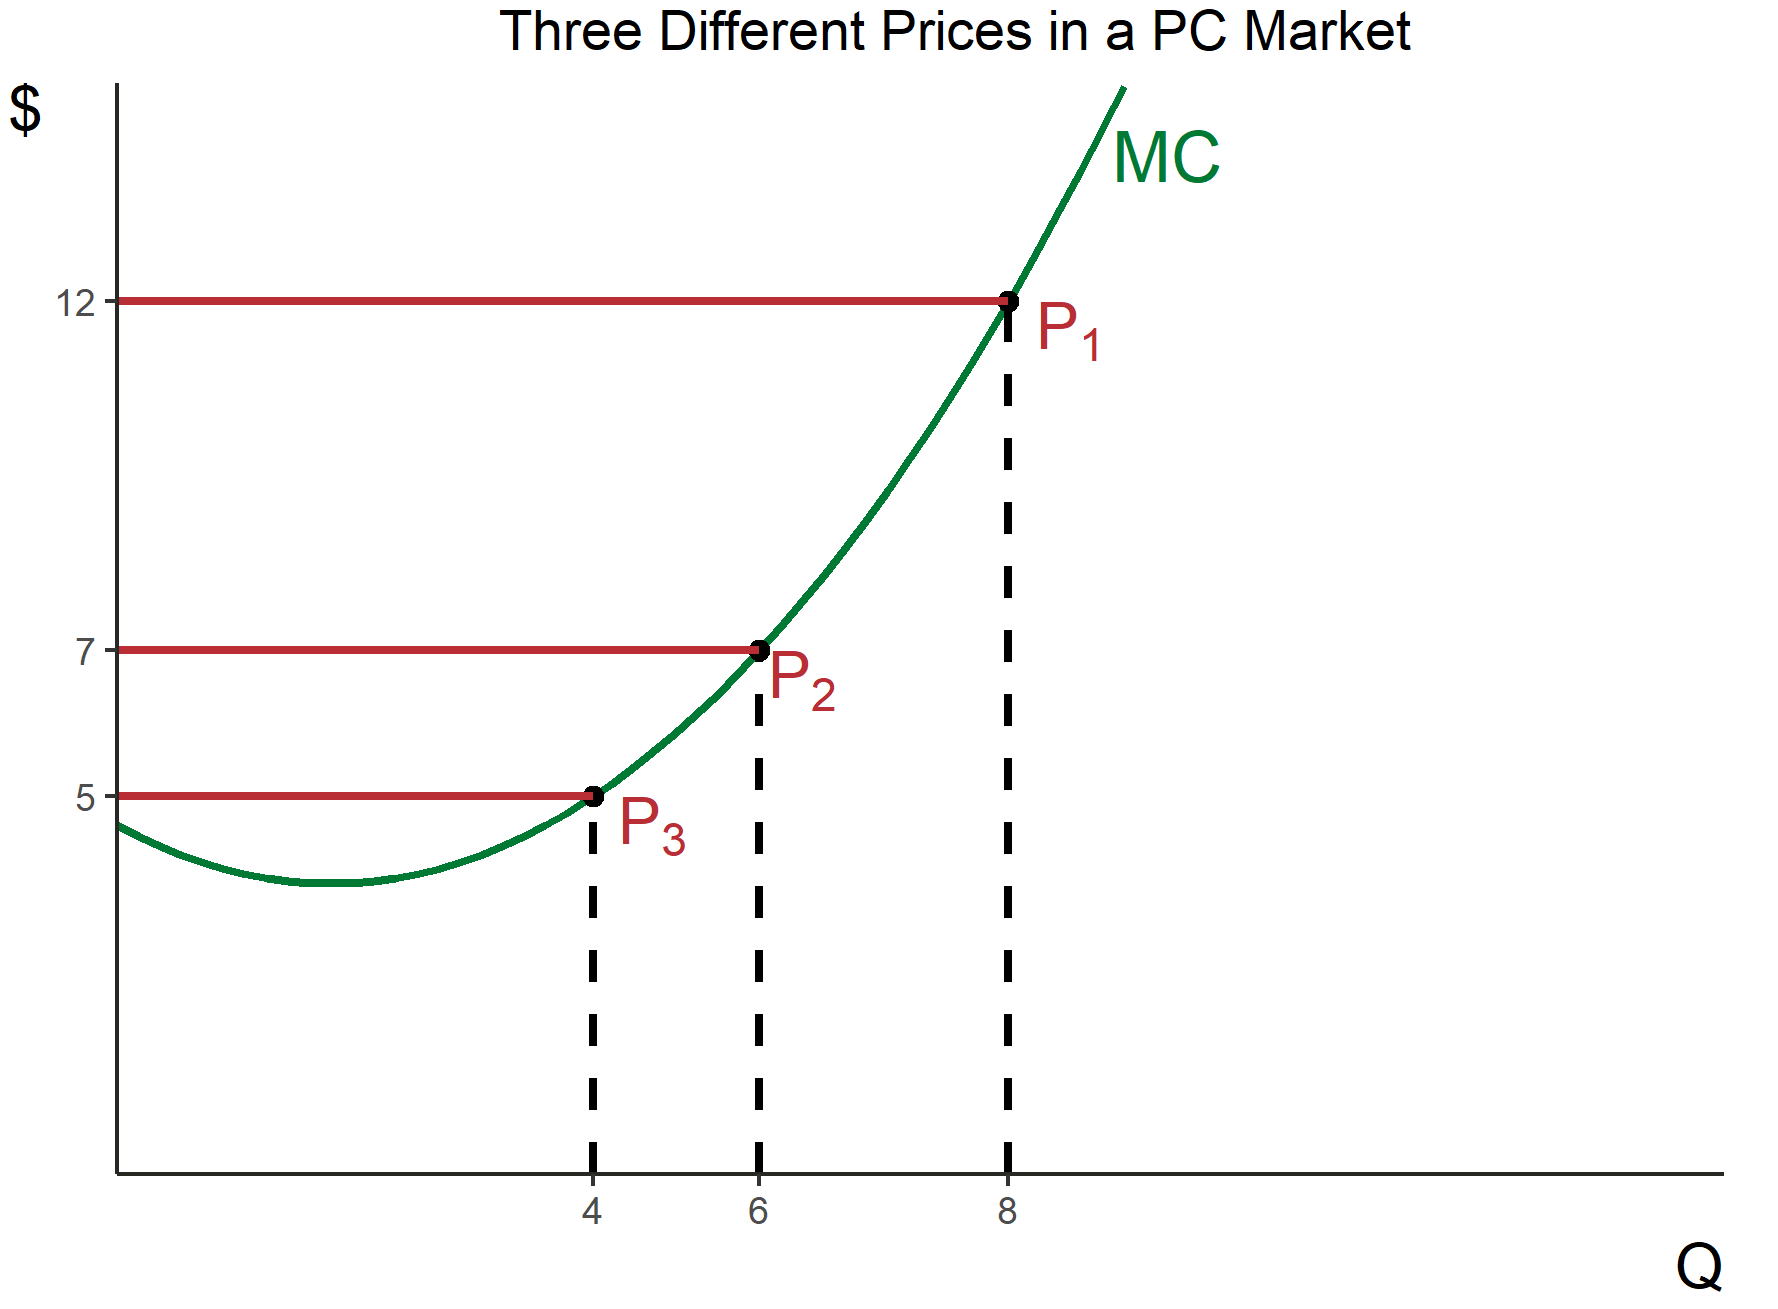
\includegraphics[width=7cm]{3 prices pc.png}
        \end{figure}
        \item What do we see?
    \end{itemize}
\end{frame}

\begin{frame}{Deriving a Firms Supply Curve}
        \begin{figure}
            \centering
            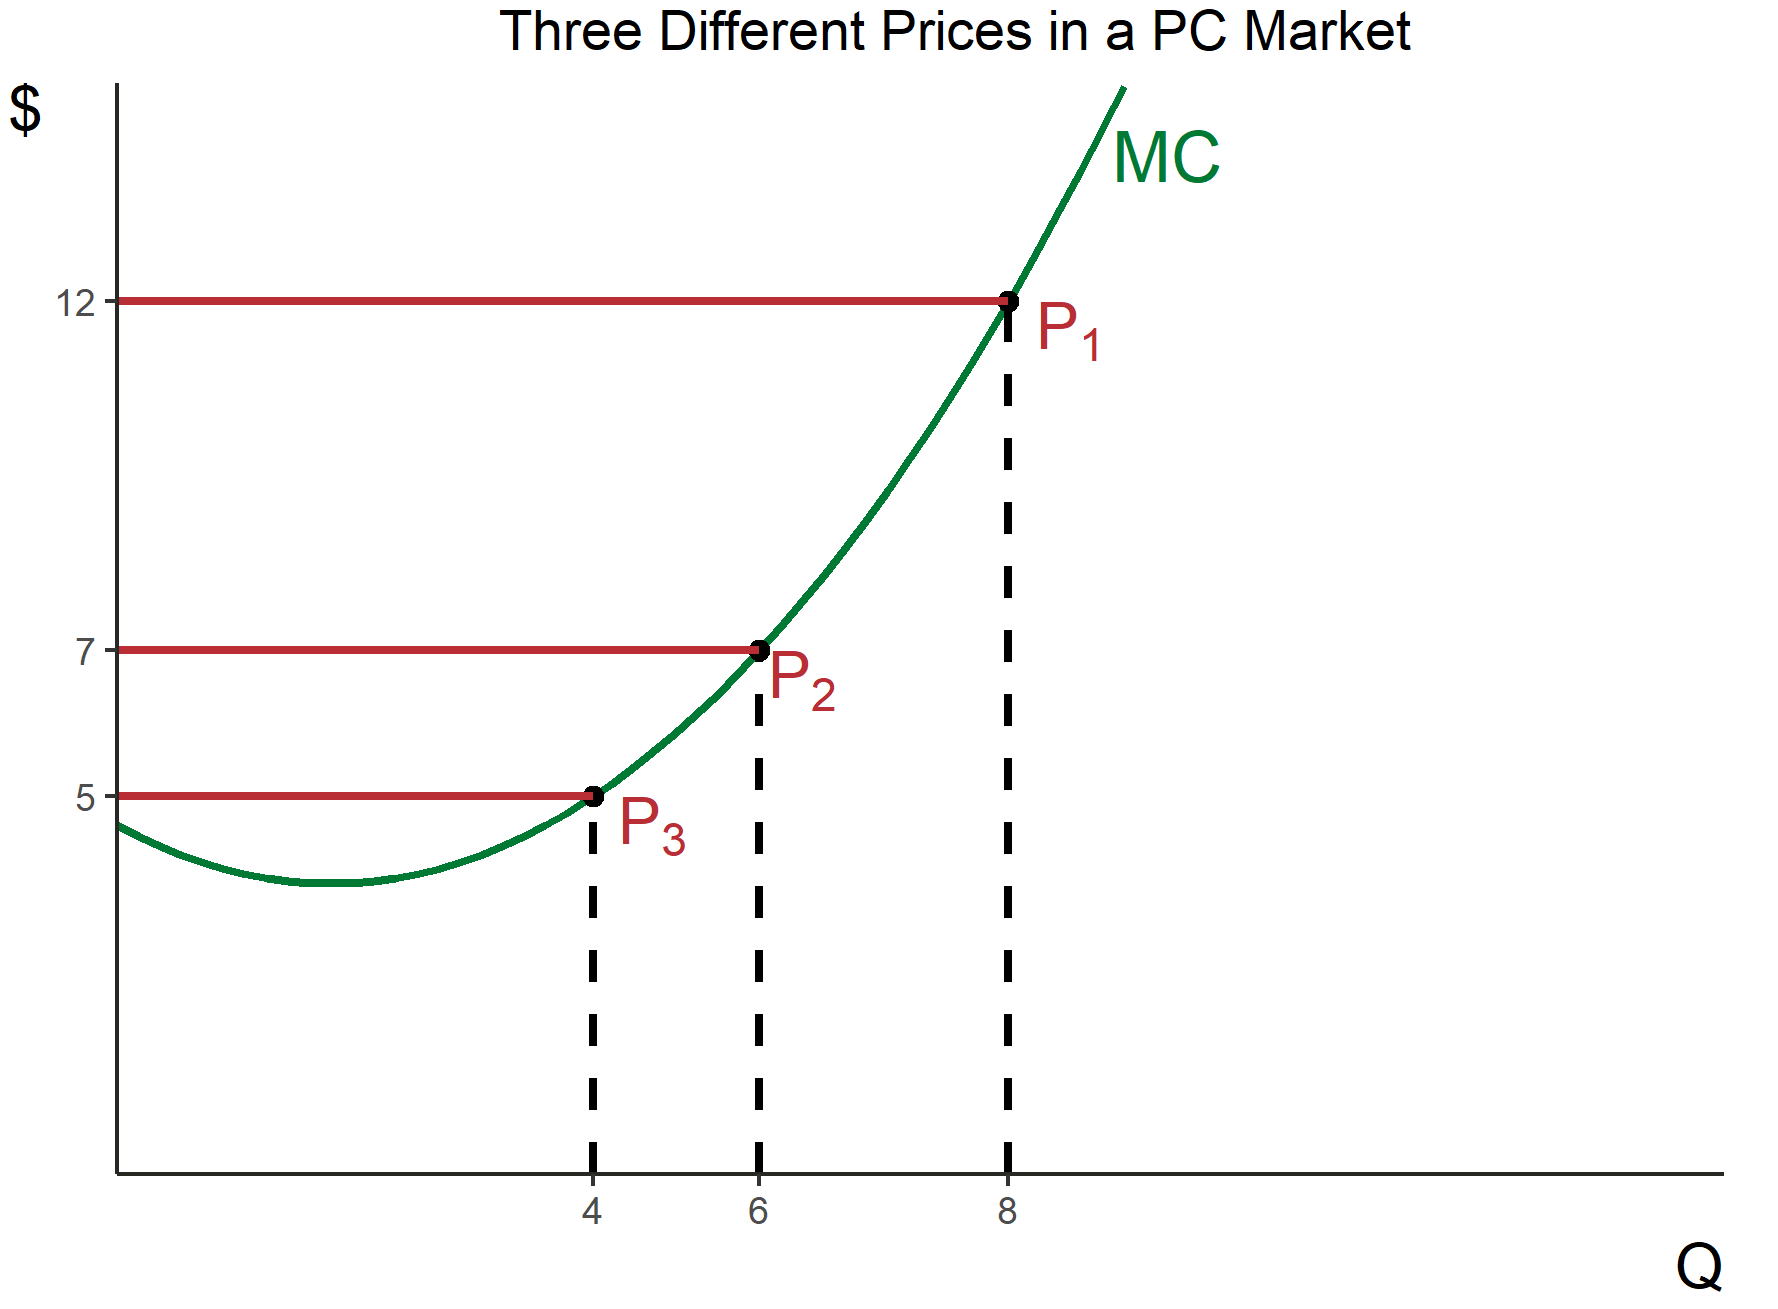
\includegraphics[width=7cm]{3 prices pc.png}
        \end{figure}
    \begin{itemize}[<+->]
        \item For each given price, the PC firm has a level they are willing to produce, based on MC
        \item So what does that make the MC curve?
        \begin{itemize}
            \item Supply!
        \end{itemize}
    \end{itemize}
\end{frame}

\begin{frame}{Deriving a Firms Supply Curve}
    \begin{itemize}[<+->]
        \item Therefore, the marginal cost curve for an individual firm is just their supply curve
        \begin{itemize}
            \item Well, not exactly -- what are we forgetting?
            \item Shutdown condition
        \end{itemize}
        \item Result: a PC firm's MC curve is exactly their SR supply curve, for values above AVC. Below AVC, their SR supply is 0 
    \end{itemize}
\end{frame}

\begin{frame}{Deriving the SR Market Supply Curve in a PC Market}
    \begin{itemize}[<+->]
        \item Once we have a bunch of firm's individual (short run) supply curves, how do we get market supply?
        \begin{itemize}
            \item Horizontal sum across supply curves
        \end{itemize}
        \item Therefore, our order of operations is 
        \begin{enumerate}
            \item Draw MC curve (or take it as given)
            \item Graph the portion of the MC curve such that $P=MC$ is above the minimum $AVC$
            \item Graph the supply curve at 0 for prices below the minimum $AVC$
            \item Horizontally sum (i.e., solve for $Q=$, and then sum) individual supply curves to get market supply
        \end{enumerate}
    \end{itemize}
\end{frame}

\begin{frame}{MC to Supply, Visually}
    \begin{itemize}[<+->]
        \item Let's start with our base firm. Note the shutdown condition point in this case:
        \begin{figure}
            \centering
            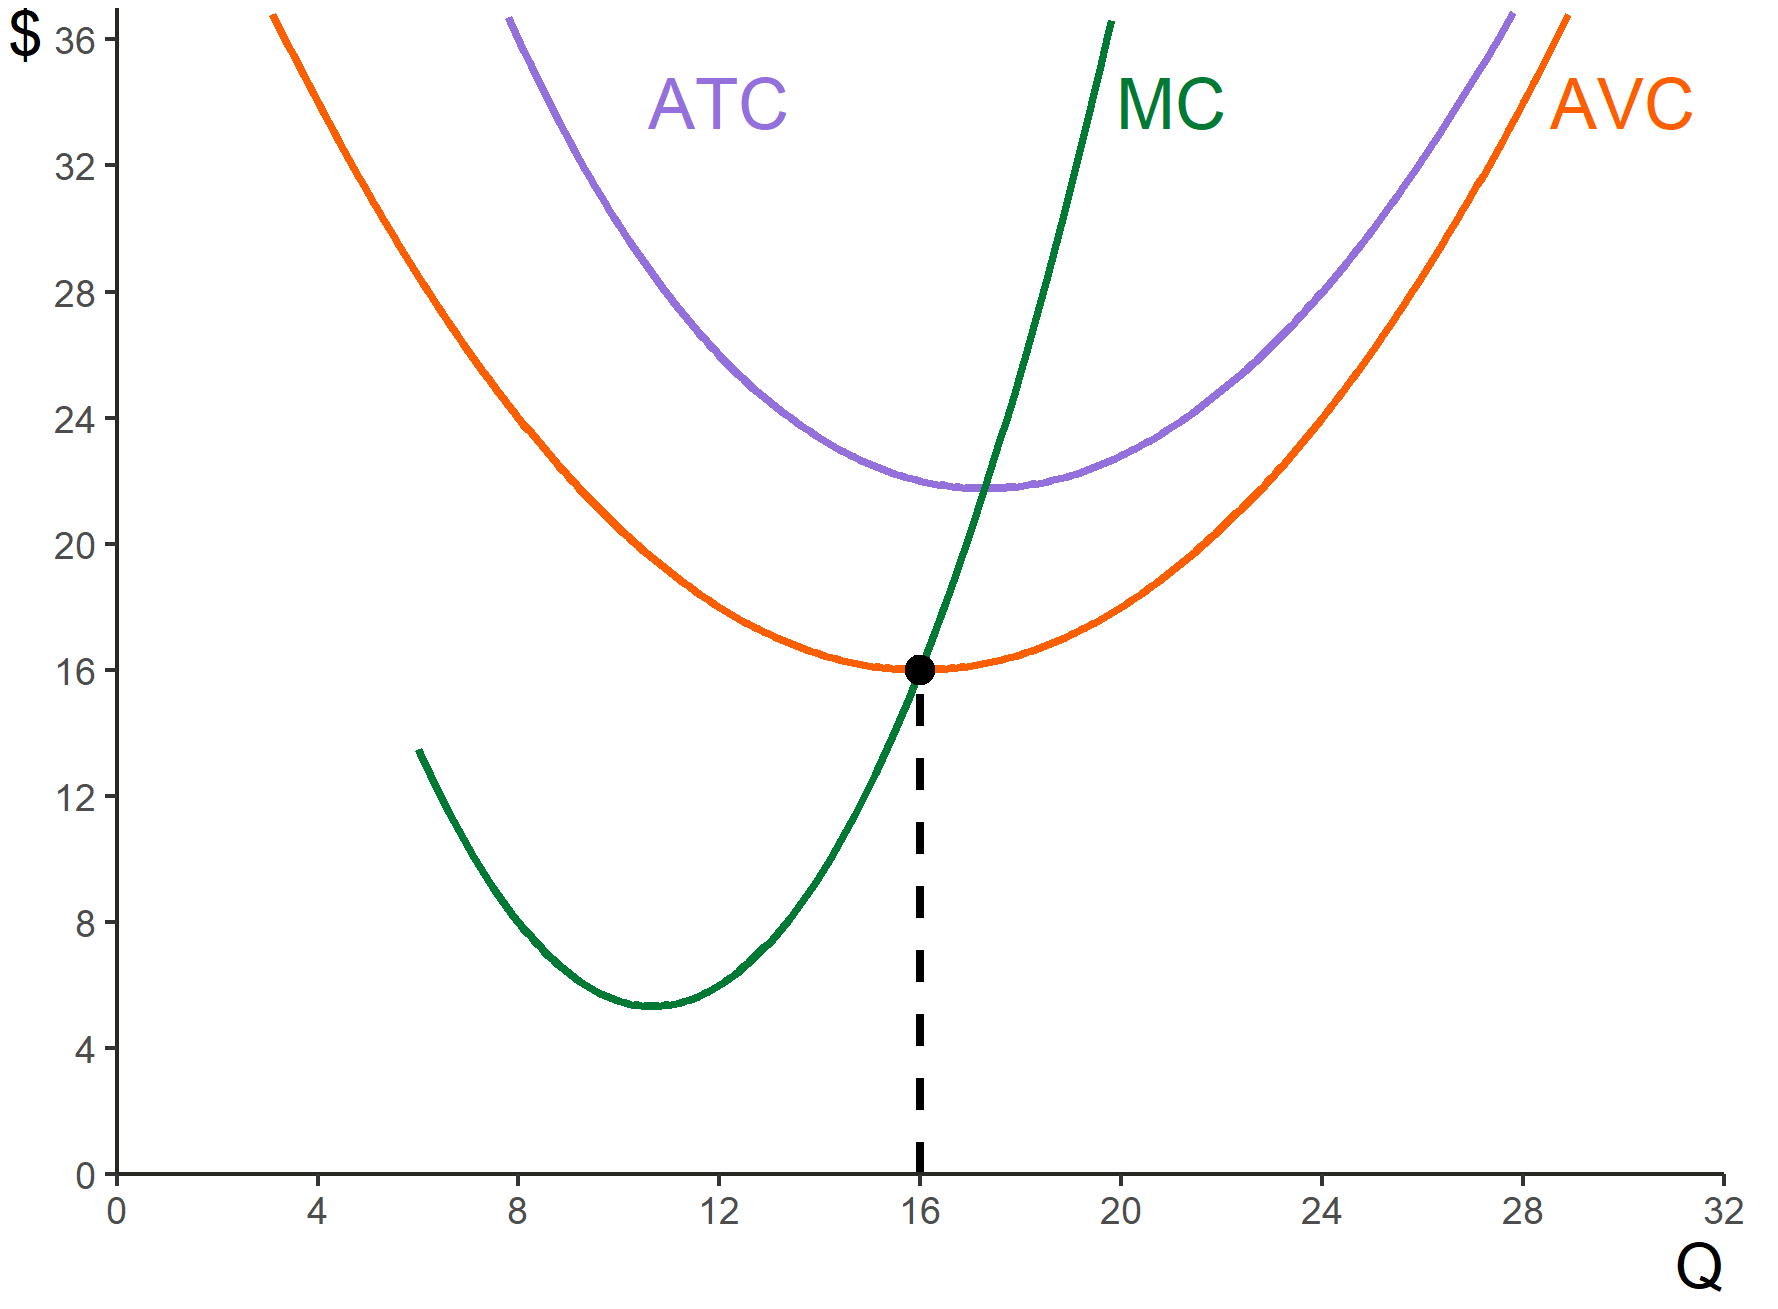
\includegraphics[width=7cm]{mc supply 1.png}
        \end{figure}
        \item Let's suppose there are 100 of such firm in the market
    \end{itemize}
\end{frame}

\begin{frame}{MC to Supply, Visually}
    \begin{itemize}[<+->]
        \item Above the shutdown point on the MC curve will become our supply curve, assuming we are producing
        \begin{figure}
            \centering
            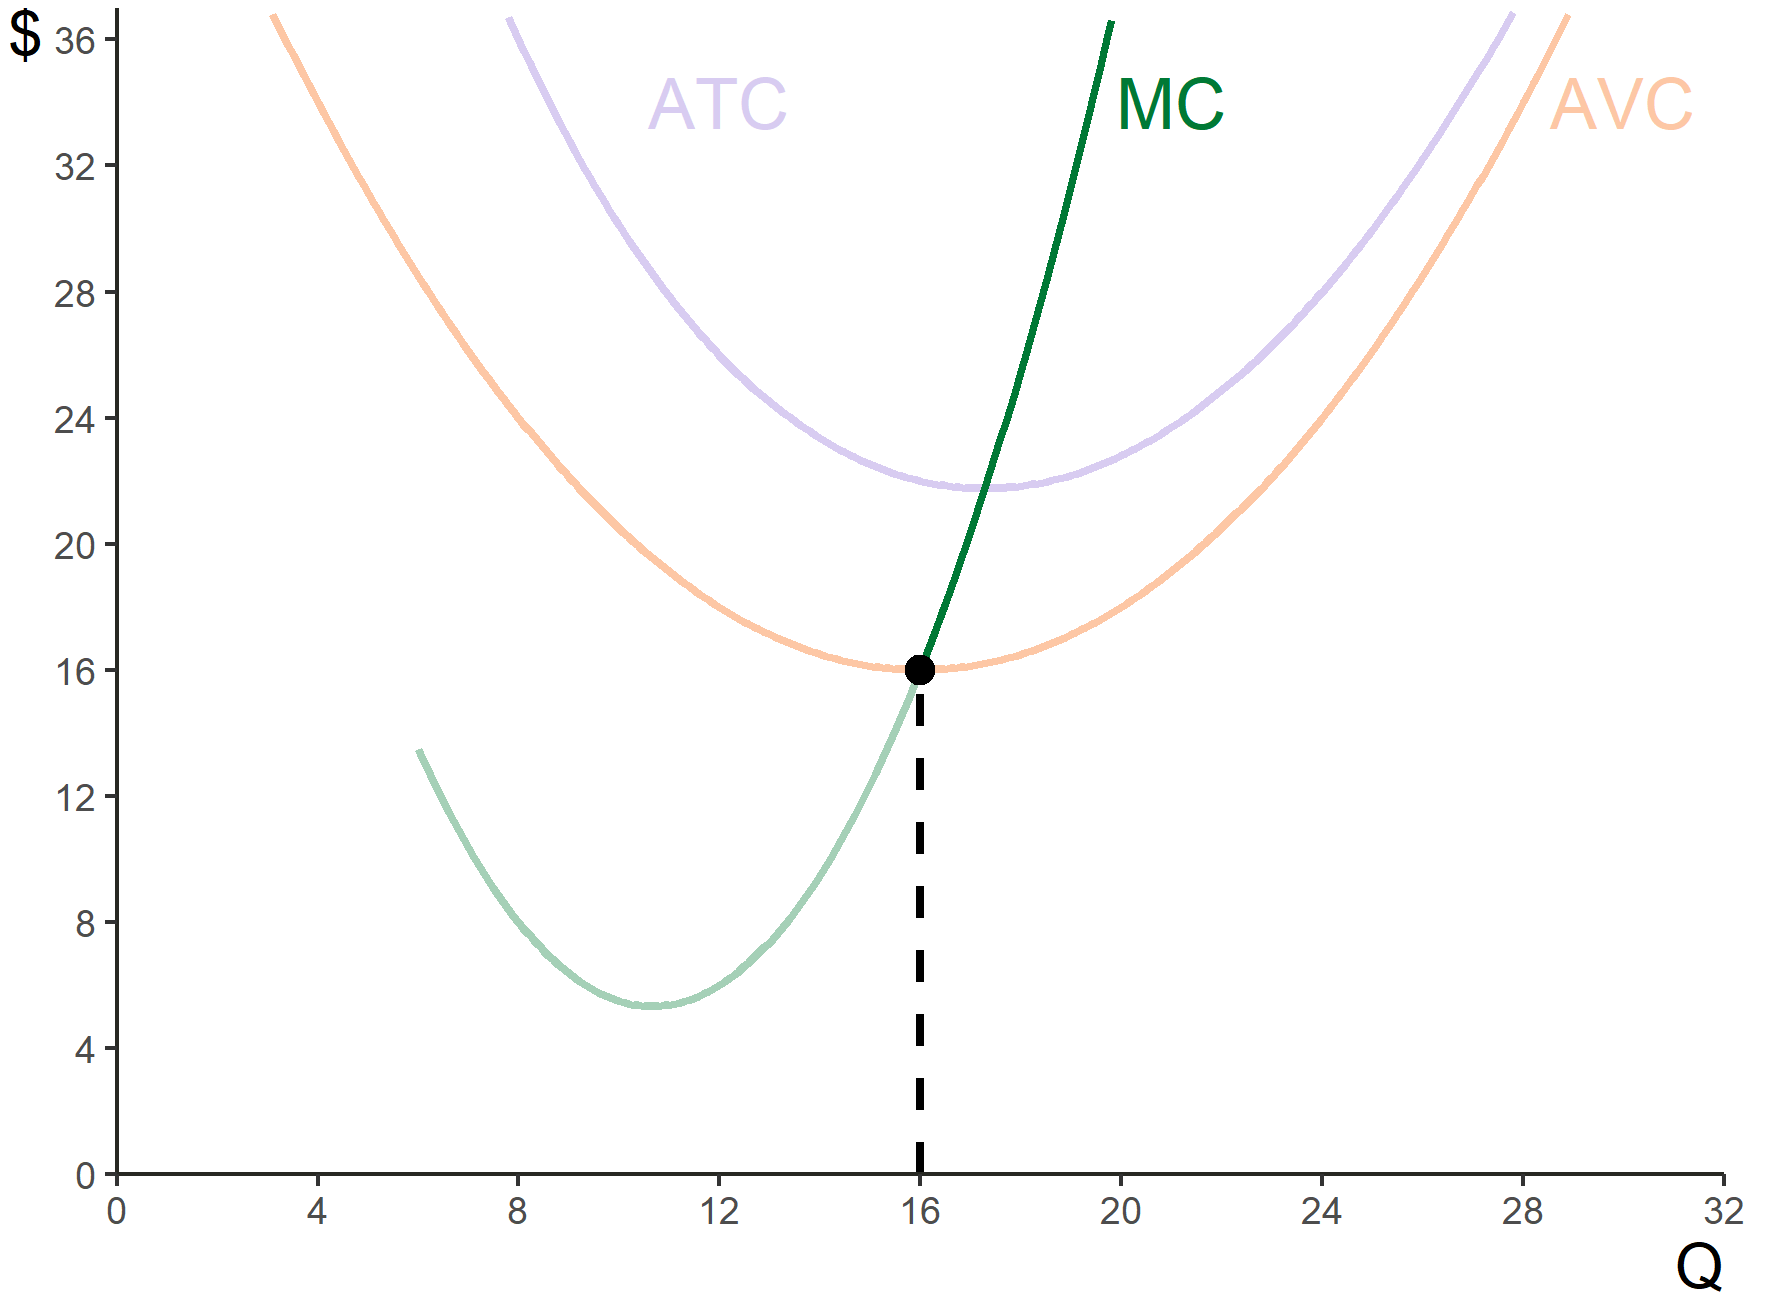
\includegraphics[width=7cm]{mc supply 2.png}
        \end{figure}
    \end{itemize}
\end{frame}

\begin{frame}{MC to Supply, Visually}
    \begin{itemize}[<+->]
        \item When we shut down, we make nothing:
        \begin{figure}
            \centering
            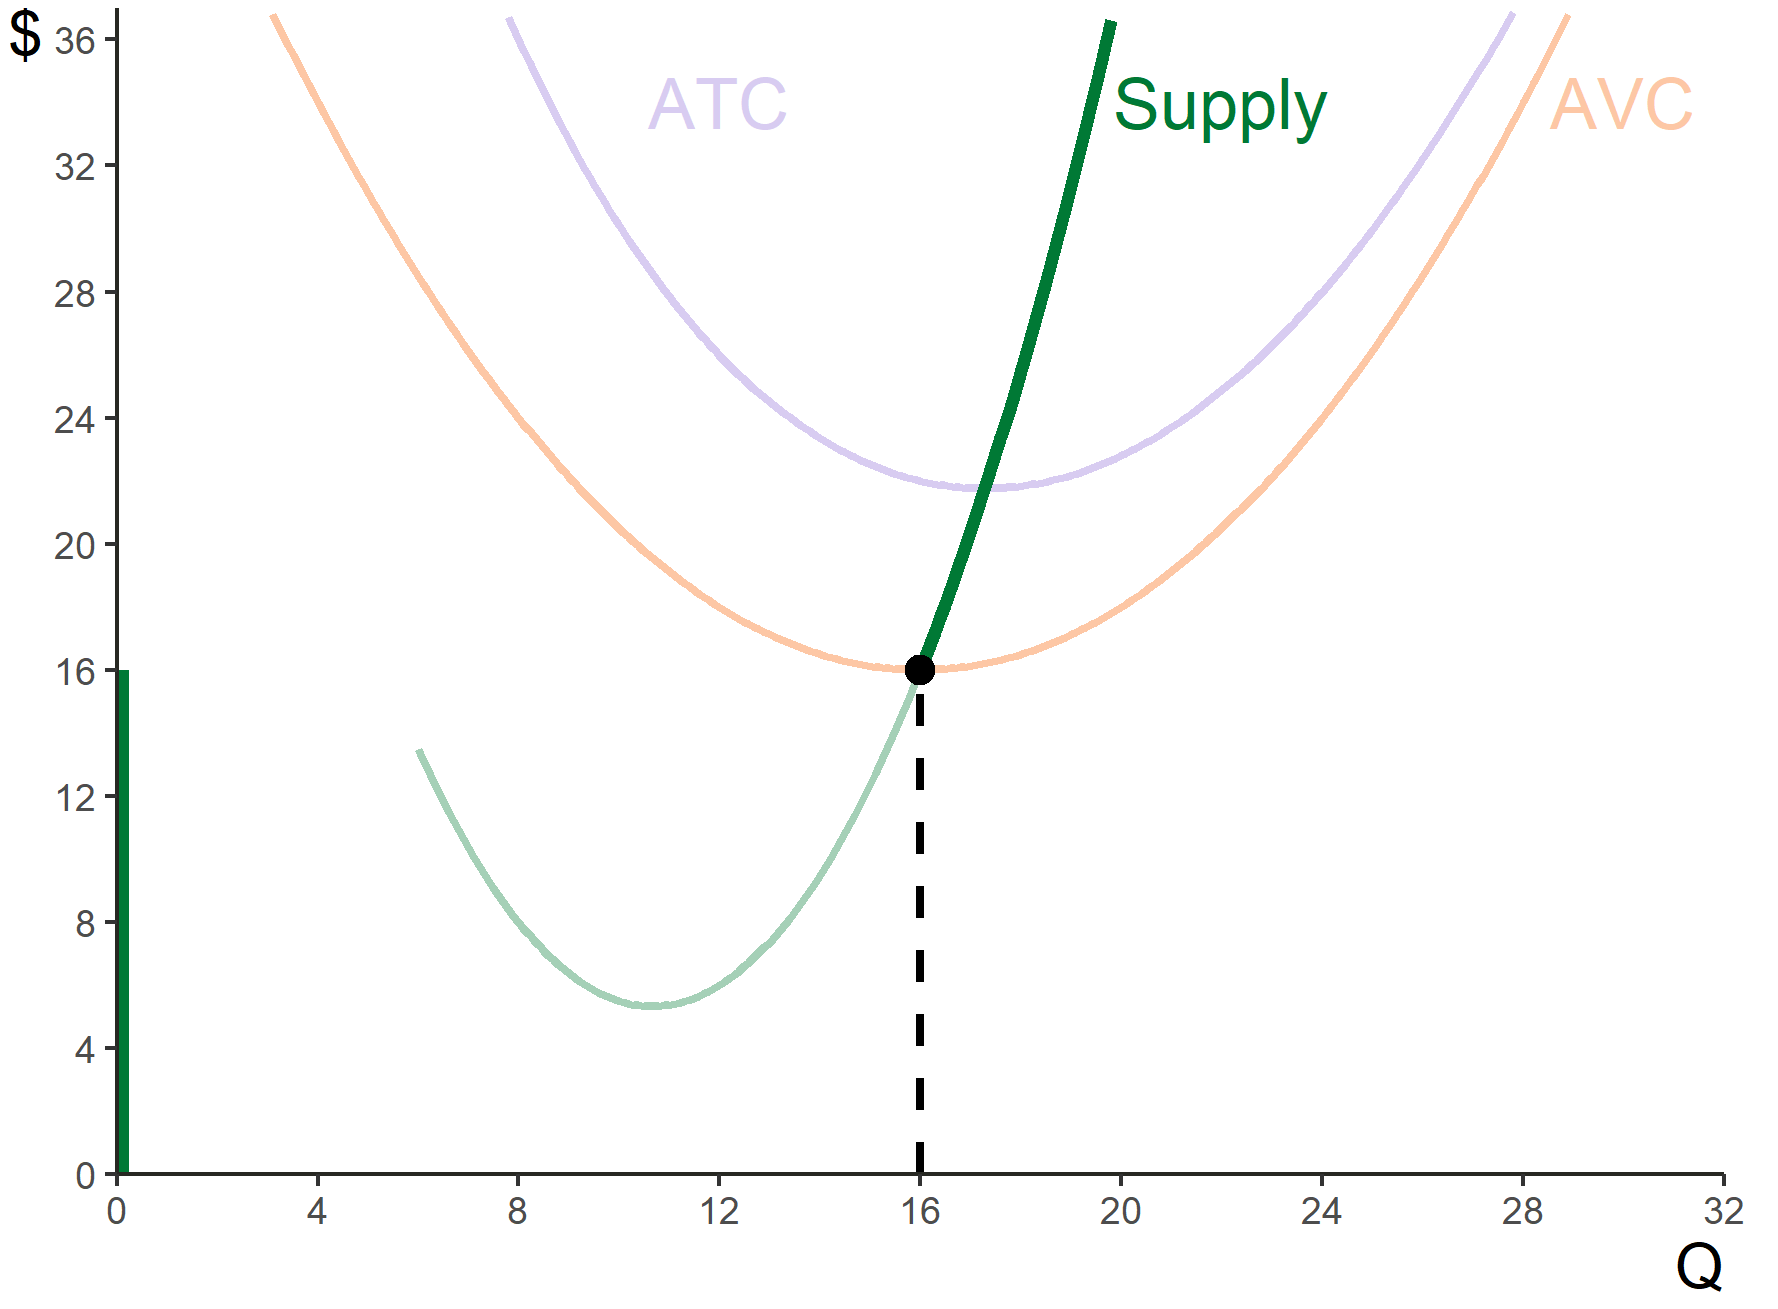
\includegraphics[width=7cm]{mc supply 3.png}
        \end{figure}
    \end{itemize}
\end{frame}

\begin{frame}{MC to Supply, Visually}
    \begin{itemize}[<+->]
        \item Therefore, our individual supply for a firm in this market is given by 
        \begin{figure}
            \centering
            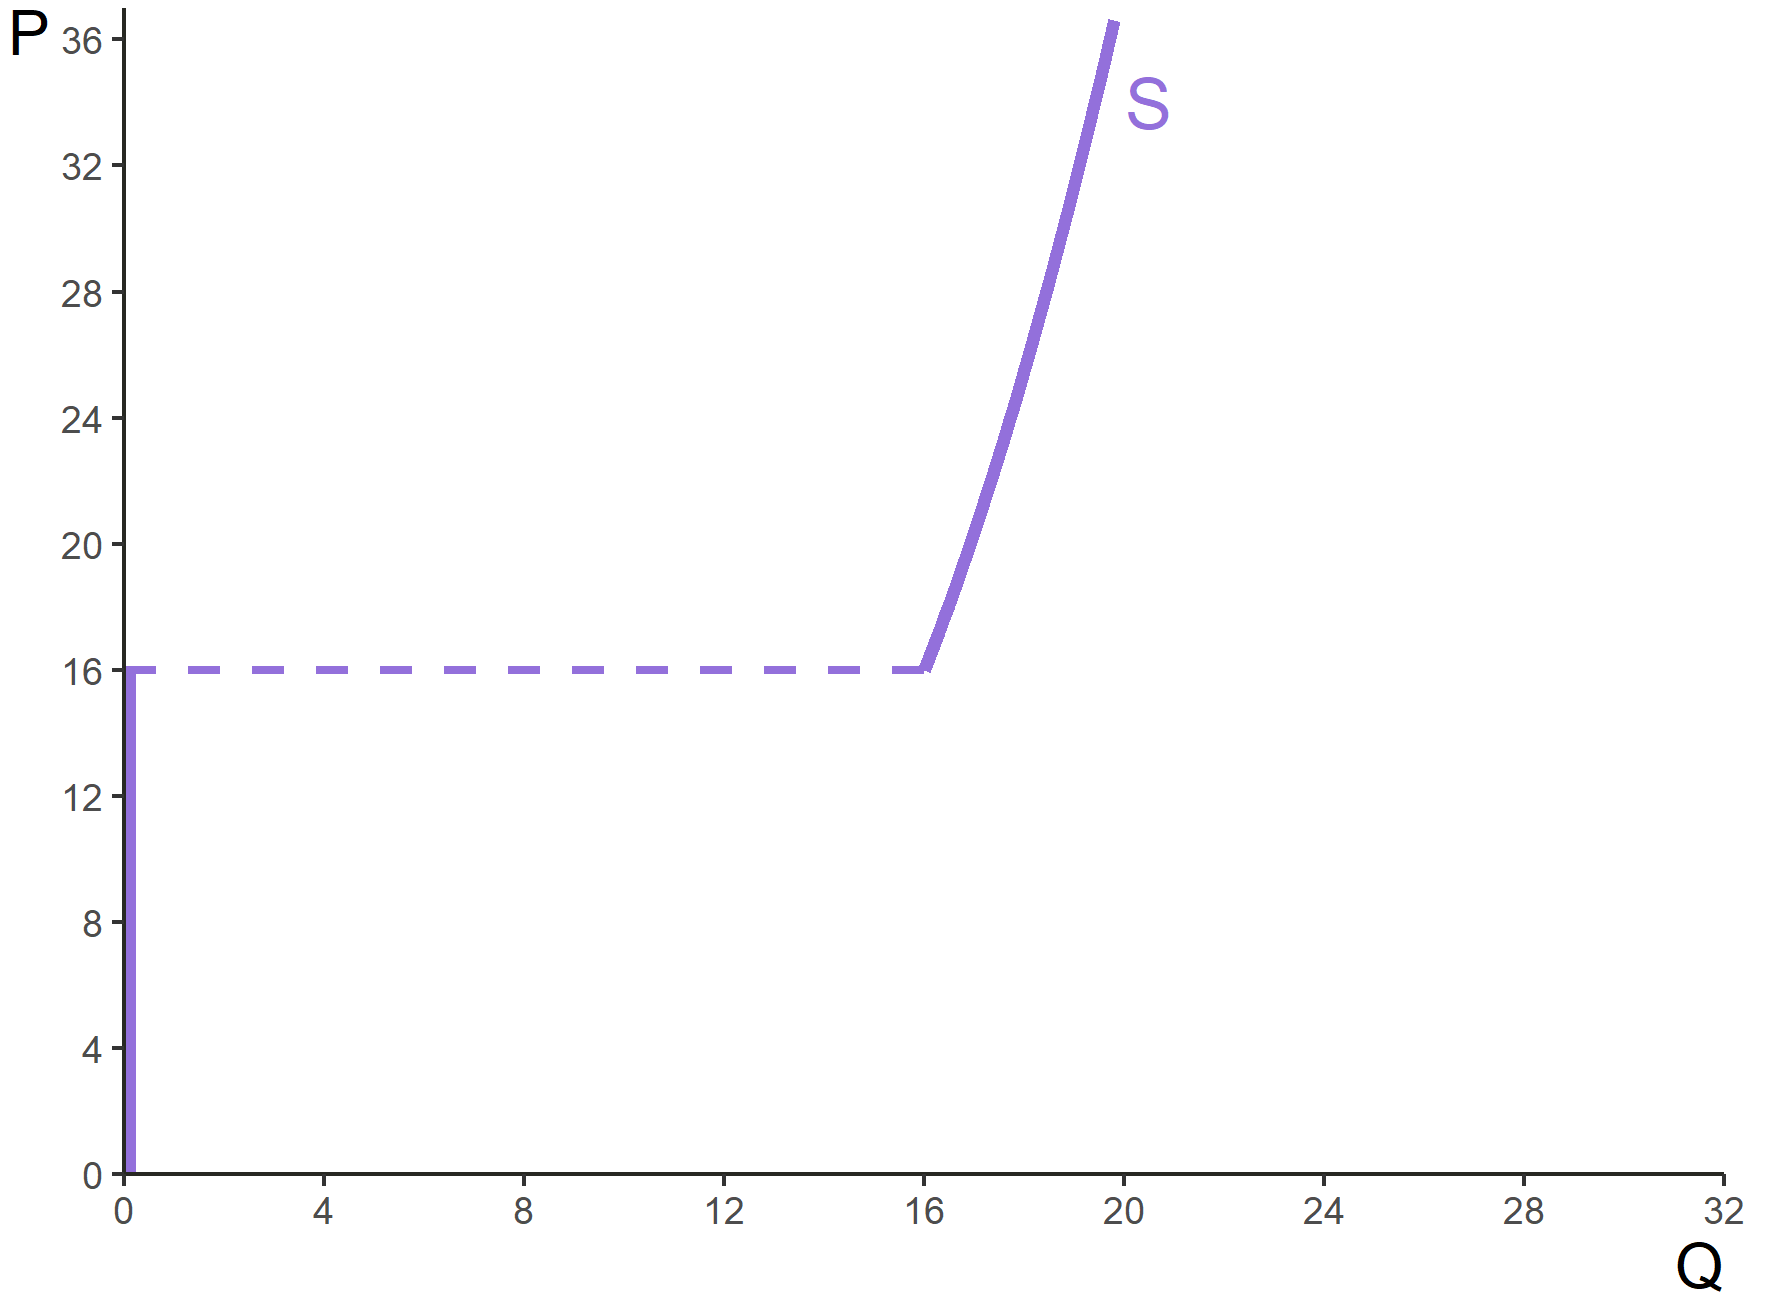
\includegraphics[width=7cm]{mc supply 4.png}
        \end{figure}
    \end{itemize}
\end{frame}

\begin{frame}{MC to Supply, Visually}
    \begin{itemize}[<+->]
        \item Since there are 100 firms, we have to take a horizontal sum of 100 such curves
        \begin{figure}
            \centering
            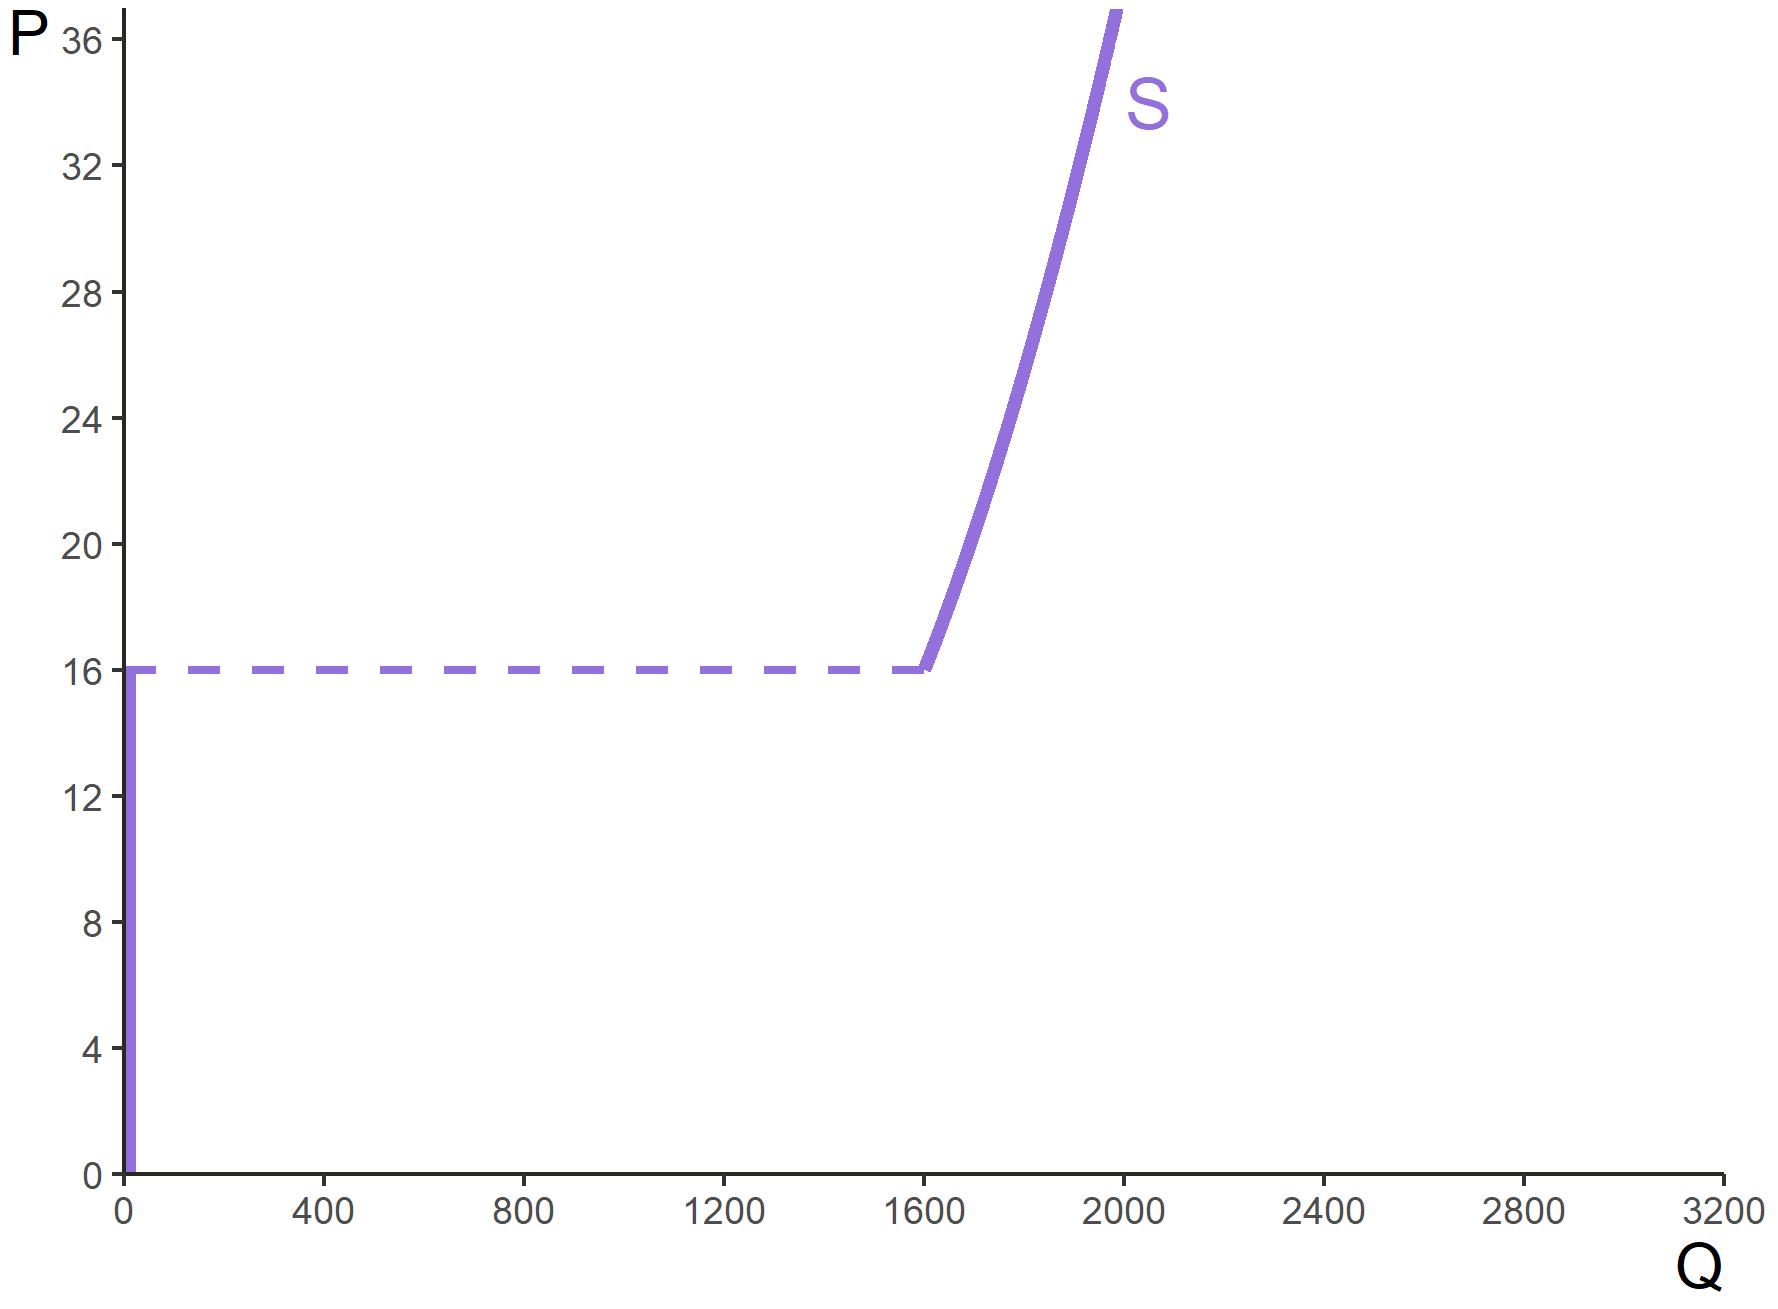
\includegraphics[width=7cm]{mc supply 5.png}
        \end{figure}
    \end{itemize}
\end{frame}

\begin{frame}{What About LR Supply?}
    \begin{itemize}[<+->]
        \item LR supply for the individual firm is very similar to the SR for the individual firm
        \item However, it will not be of concern to draw the LR individual supply curve for the individual firm, but if you wanted to:
        \begin{itemize}
            \item The firm shuts down in the long run if $P<LRATC$, so the LR individual supply curve will be equal to MC above this point, and 0 (or, in this case, non-existent) below it
        \end{itemize}
        \item The real importance is in the long run supply curve for the market
    \end{itemize}
\end{frame}

\begin{frame}{What About LR Supply?}
    \begin{itemize}[<+->]
        \item How does the narrative for market supply change in the long run? 
        \item In the long run, firms' economic profit is 0
        \item Firms have no incentive to enter or leave, so there is no reason for a price movement
        \item Even if there was a price movement:
        \begin{itemize}
            \item If the the \textit{long-run} price is lowered, many producers will drop out of the market, unless they can invent new technology (as they are currently breaking even, and this would cause profits to drop)
            \item If the \textit{long-run} price is raised, we would see endless entry into the market (or, you could just say that this is impossible: the price will be driven back down)
        \end{itemize}
        \item In other words, long run market supply is \textit{infinitely sensitive} to changes in the price
        \item So what does long run supply look like?
        \begin{itemize}
            \item Perfectly elastic -- flat
        \end{itemize}
    \end{itemize}
\end{frame}

\begin{frame}{Long Run Market Supply Curve}
    \begin{itemize}[<+->]
        \item In a market with identical firms, the zero-profit (break-even) point for a particular firm defines the long-run supply curve in the market
        \begin{figure}
            \centering
            \includegraphics<1>[width=10cm]{lr supply1.png}
        \end{figure}
    \end{itemize}
\end{frame}




\section*{S\&D Example}

\begin{frame}{An Observation\footnote{Some people make this point more strongly than others. It doesn't affect our discussion that much, but it is still worth mentioning.}}
    \begin{itemize}[<+->]
        \item From an individual firm's perspective:
        \begin{itemize}
            \item If I raise my prices, consumers drop out of the market
            \item If I lower my prices, I will capture the market, but be producing so much that I accrue too much loss and are forced to drop out of the market
        \end{itemize}
        \item So what does demand look like to the PC firm?
        \begin{itemize}
            \item Infinitely sensitive to changes in price aka perfectly elastic
        \end{itemize}
        \item This is just from the firm's perspective: this is why the price line is flat: they perceive demand is perfectly elastic, when they are in fact the ones that 
        \item In reality, market demand in a PC market is still downward sloping
    \end{itemize}
\end{frame}

\begin{frame}{Linear Example}
    \begin{itemize}[<+->]
        \item Let's walk through a full example of the relationships going on in this market
        \item We will use mostly linear curves, which will take care of a lot of our problems
        \begin{itemize}
            \item Namely, recall that linear MC and AVC curves means that our shutdown condition happens exactly when the firm will choose to produce $Q=0$ anyway
        \end{itemize}
        \item I won't dive into the numbers, but I'll provide them for reference
    \end{itemize}
\end{frame}

\begin{frame}{Linear Example}
    \begin{itemize}[<+->]
        \item To start, let's assume that there are 50 firms in the market, with
        \begin{align*}
            [MC]&:\qquad 10+\frac{9}{10}Q\\
            [AVC]&:\qquad 10+\frac{9}{20}Q\\
            [FC]&:\qquad 45
        \end{align*}
        \item To start, try finding the equations for our other objects of interest: TC, ATC, VC, AFC
        \begin{multicols}{2}
            \begin{itemize}
                \item $VC=10Q+\frac{9}{20}Q^{2}$
                \item $TC=10Q+\frac{9}{20}Q^{2}+45$
                \item $ATC=10+\frac{9}{20}Q+\frac{45}{Q}$
                \item $AFC=\frac{45}{Q}$
            \end{itemize}
        \end{multicols}
        \item What will these objects look like?
    \end{itemize}
\end{frame}

\begin{frame}{Representative Firm}
    \begin{itemize}[<+->]
        \item Next, let's try to graph MC, AVC, and ATC for a representative firm:
        \begin{figure}
            \centering
            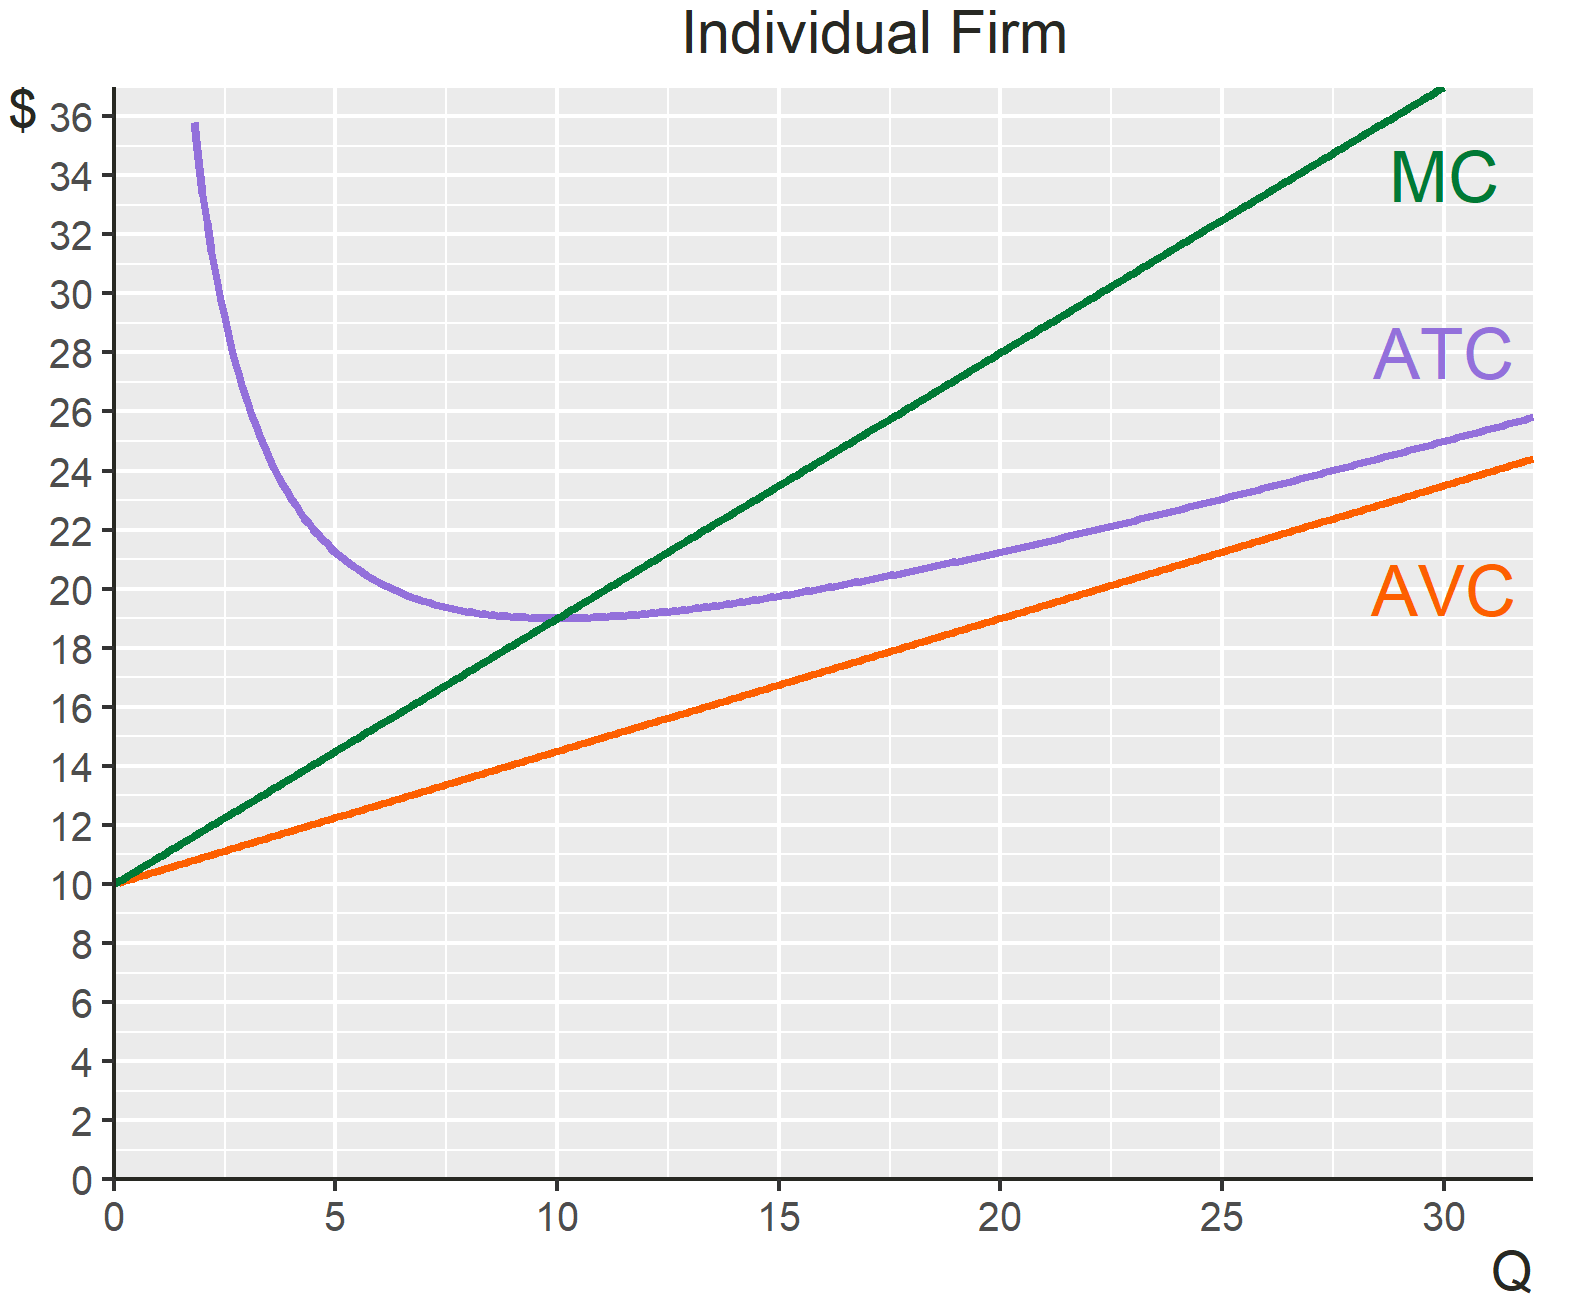
\includegraphics[width=8cm]{linex1.png}
        \end{figure}
    \end{itemize}
\end{frame}

\begin{frame}{Shutdown Condition}
        \begin{figure}
            \centering
            \includegraphics[width=7cm]{Rplot.pdf}\vspace{-4mm}
        \end{figure}
    \begin{itemize}[<+->]
        \item When will the firm shut down?
        \begin{itemize}
            \item In the short run, only when $P<10$: the firm would not produce for less than this anyway, so there is effectively no SR shutdown condition
            \item In the long run, exit when $P<19$
        \end{itemize}
    \end{itemize}
\end{frame}

\begin{frame}{Shutdown Condition}
        \begin{figure}
            \centering
            \includegraphics[width=7cm]{Rplot.pdf}\vspace{-3mm}
        \end{figure}
    \begin{itemize}[<+->]
        \item Where is the break-even point?
        \begin{itemize}
            \item Where ATC intersects MC: $(10,19)$
        \end{itemize}
    \end{itemize}
\end{frame}

\begin{frame}{Market Supply}
    \begin{itemize}[<+->]
        \item This induces the following SR and LR supply curves:
        \begin{center}
            \hbox{\hspace{0.9em}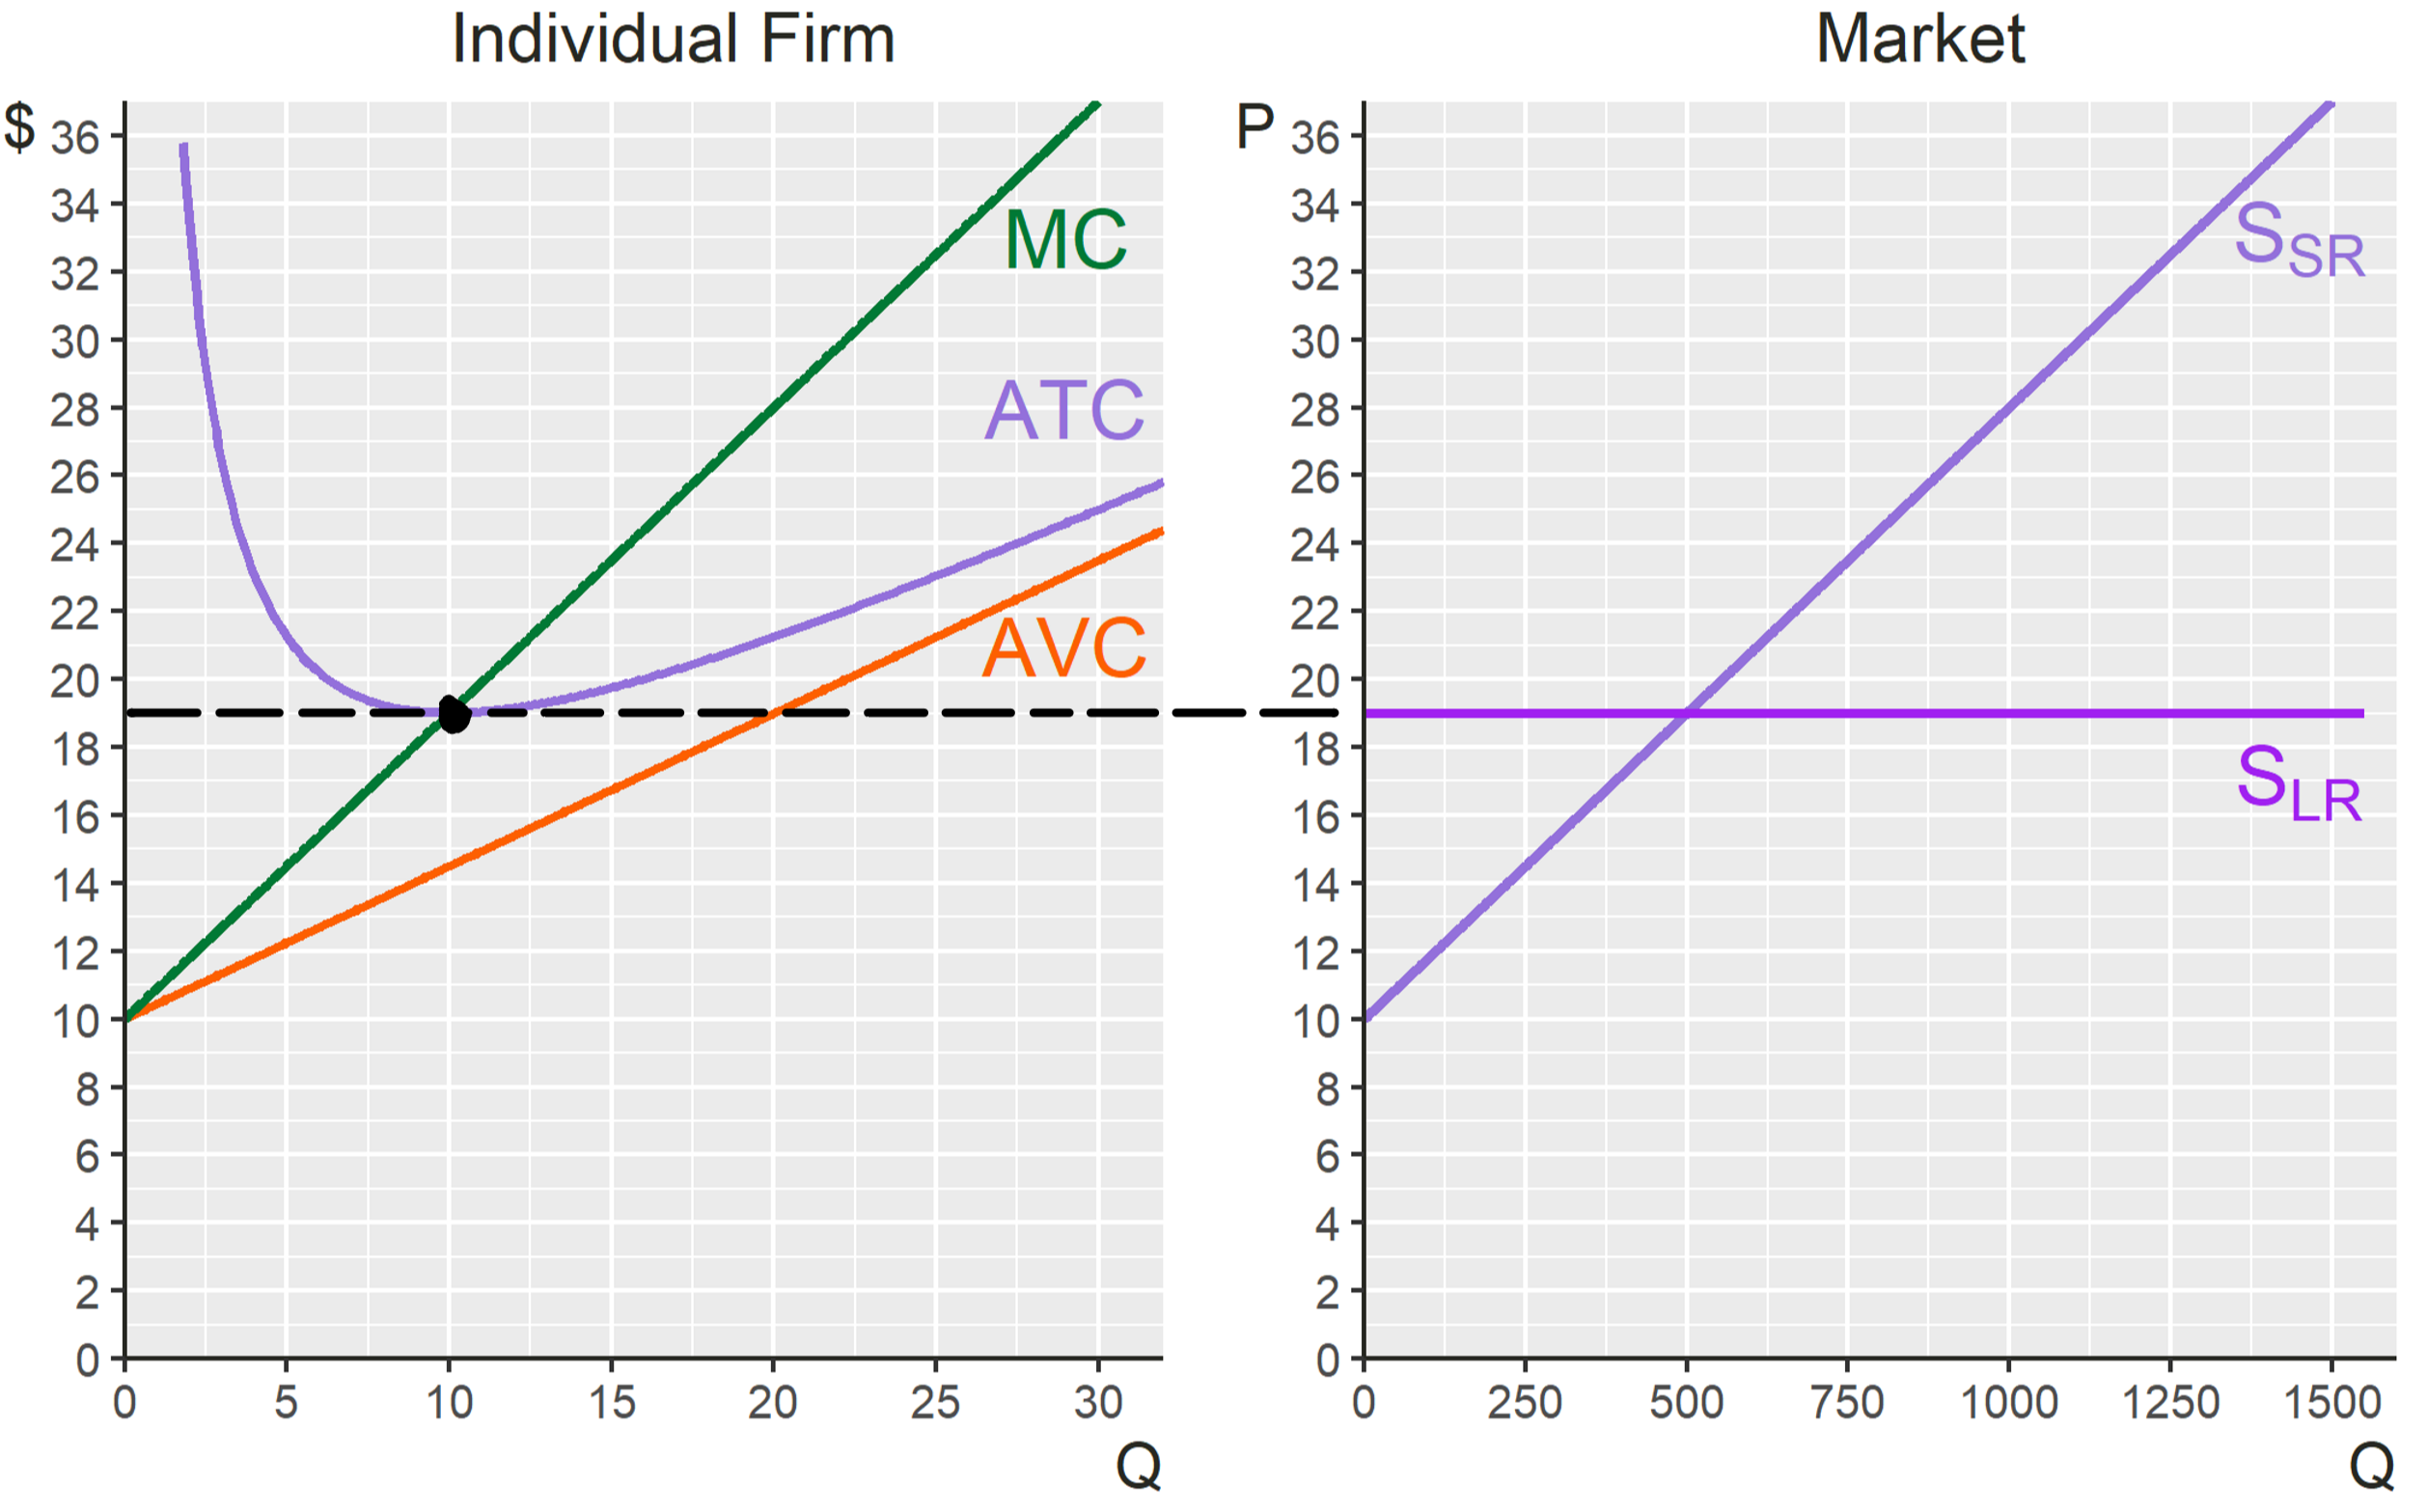
\includegraphics[width=11cm]{linex3.png}}
        \end{center}
    \end{itemize}
\end{frame}

\begin{frame}{Adding Demand}
    \begin{itemize}[<+->]
        \item Now let's consider a couple of demand curves
        \item Demand curves in the market induce $P=MR$ lines for the individual firm
        \begin{figure}
            \centering
            \hbox{\hspace{0.9em}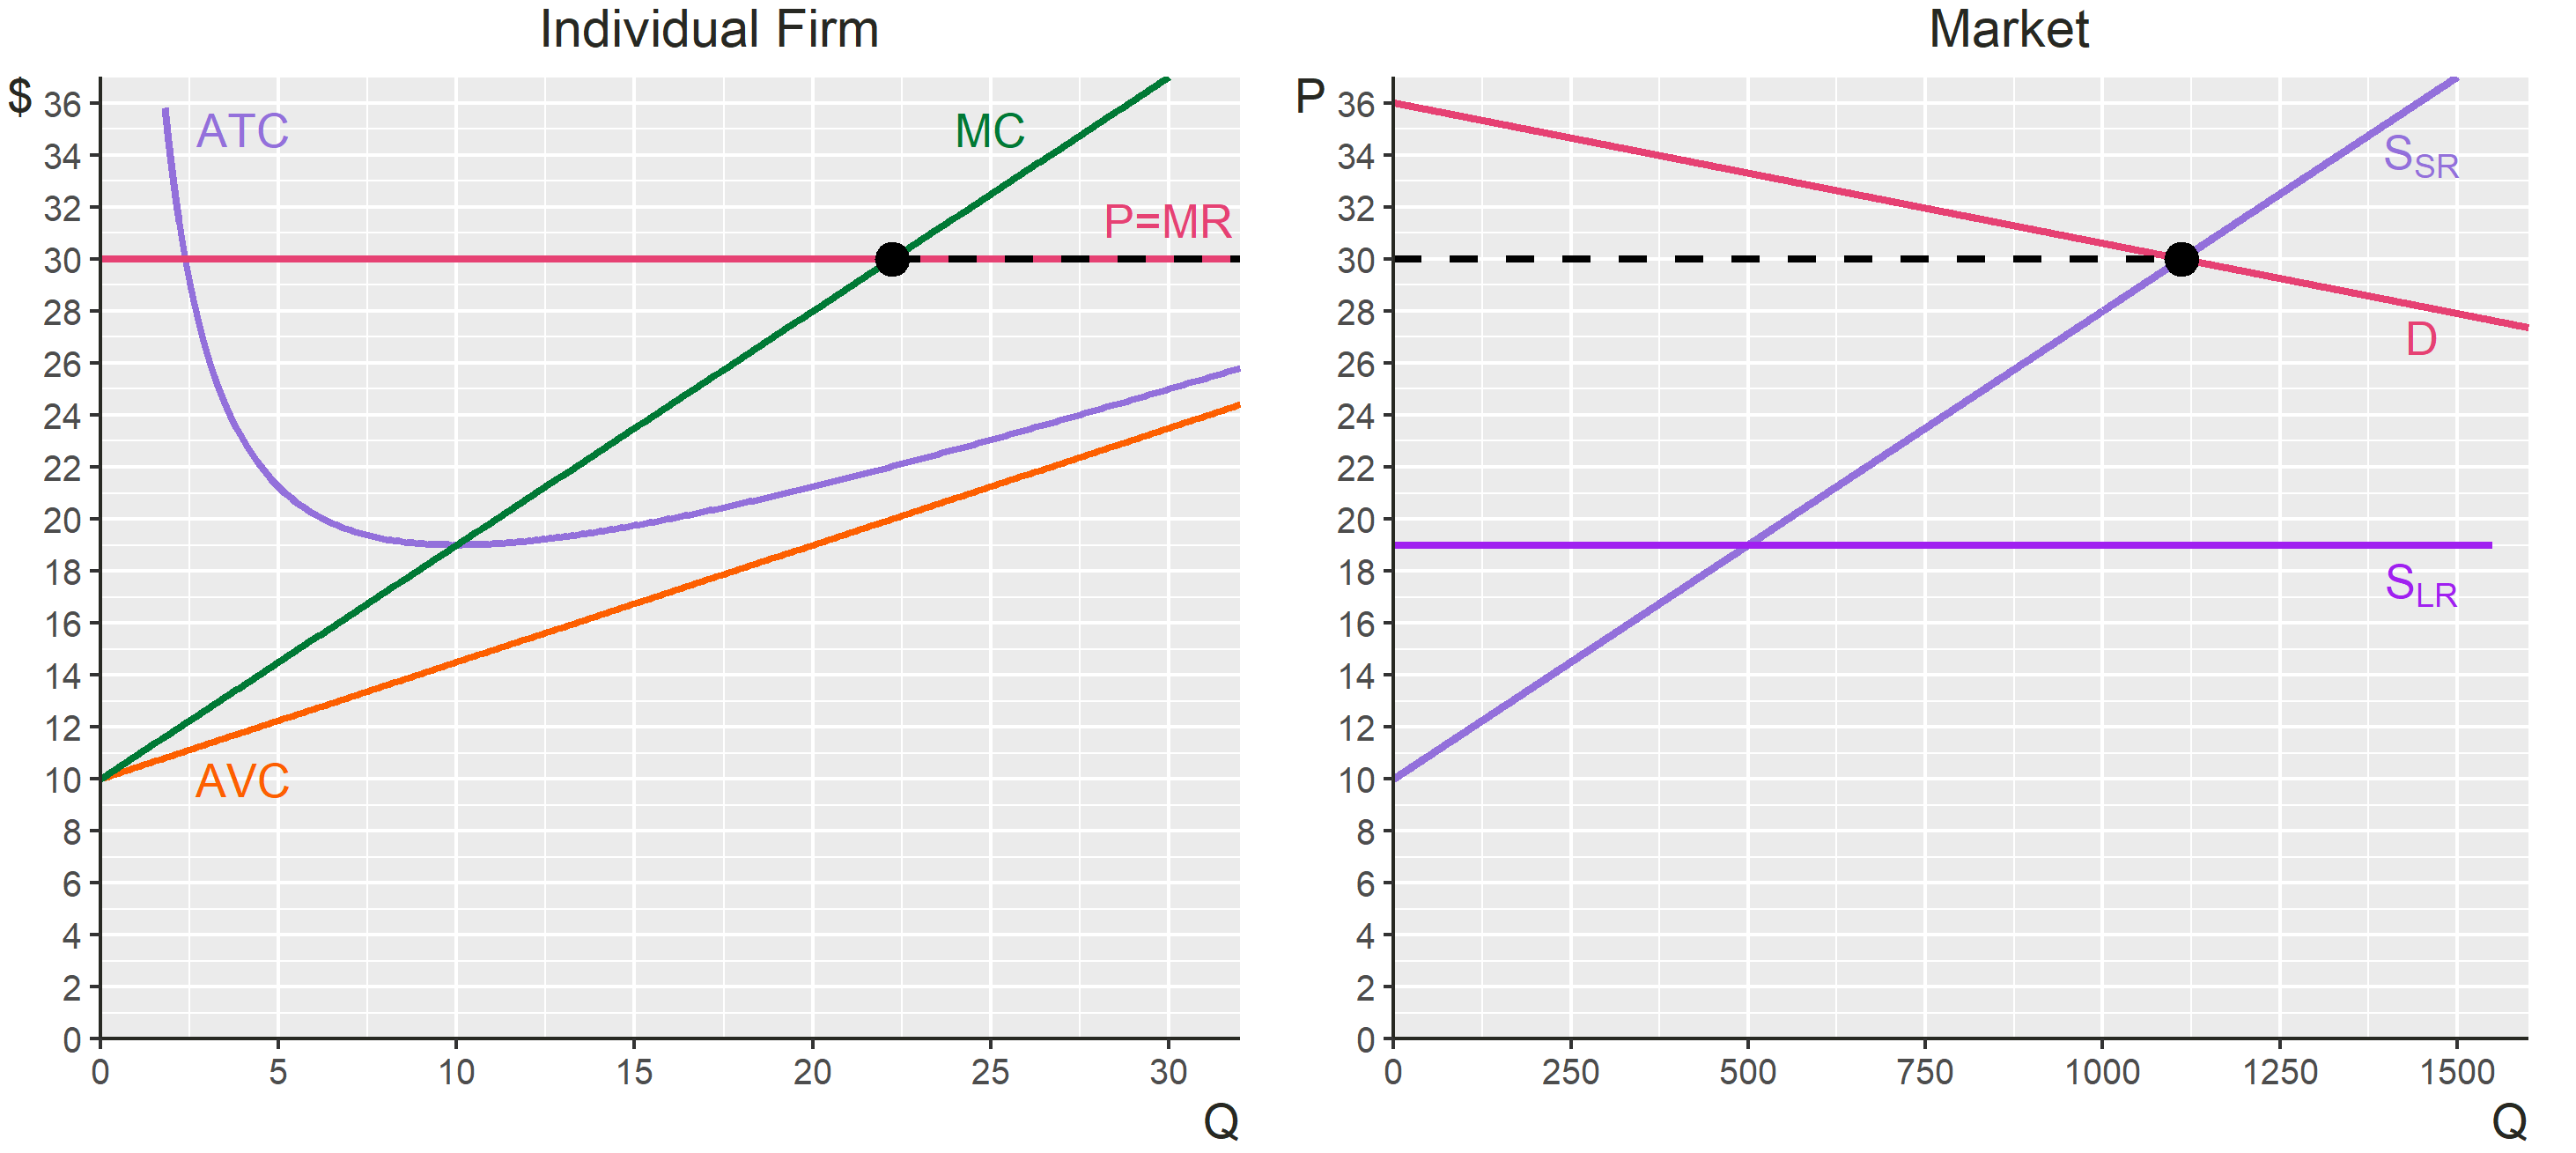
\includegraphics[width=11cm]{linex4.png}}
        \end{figure}
    \end{itemize}
\end{frame}

\begin{frame}{Equilibria}
    \begin{itemize}[<+->]
        \item Note that the following demand curve induces both a short and long run equilibrium. Why?
        \begin{figure}
            \centering
            \hbox{\hspace{0.9em}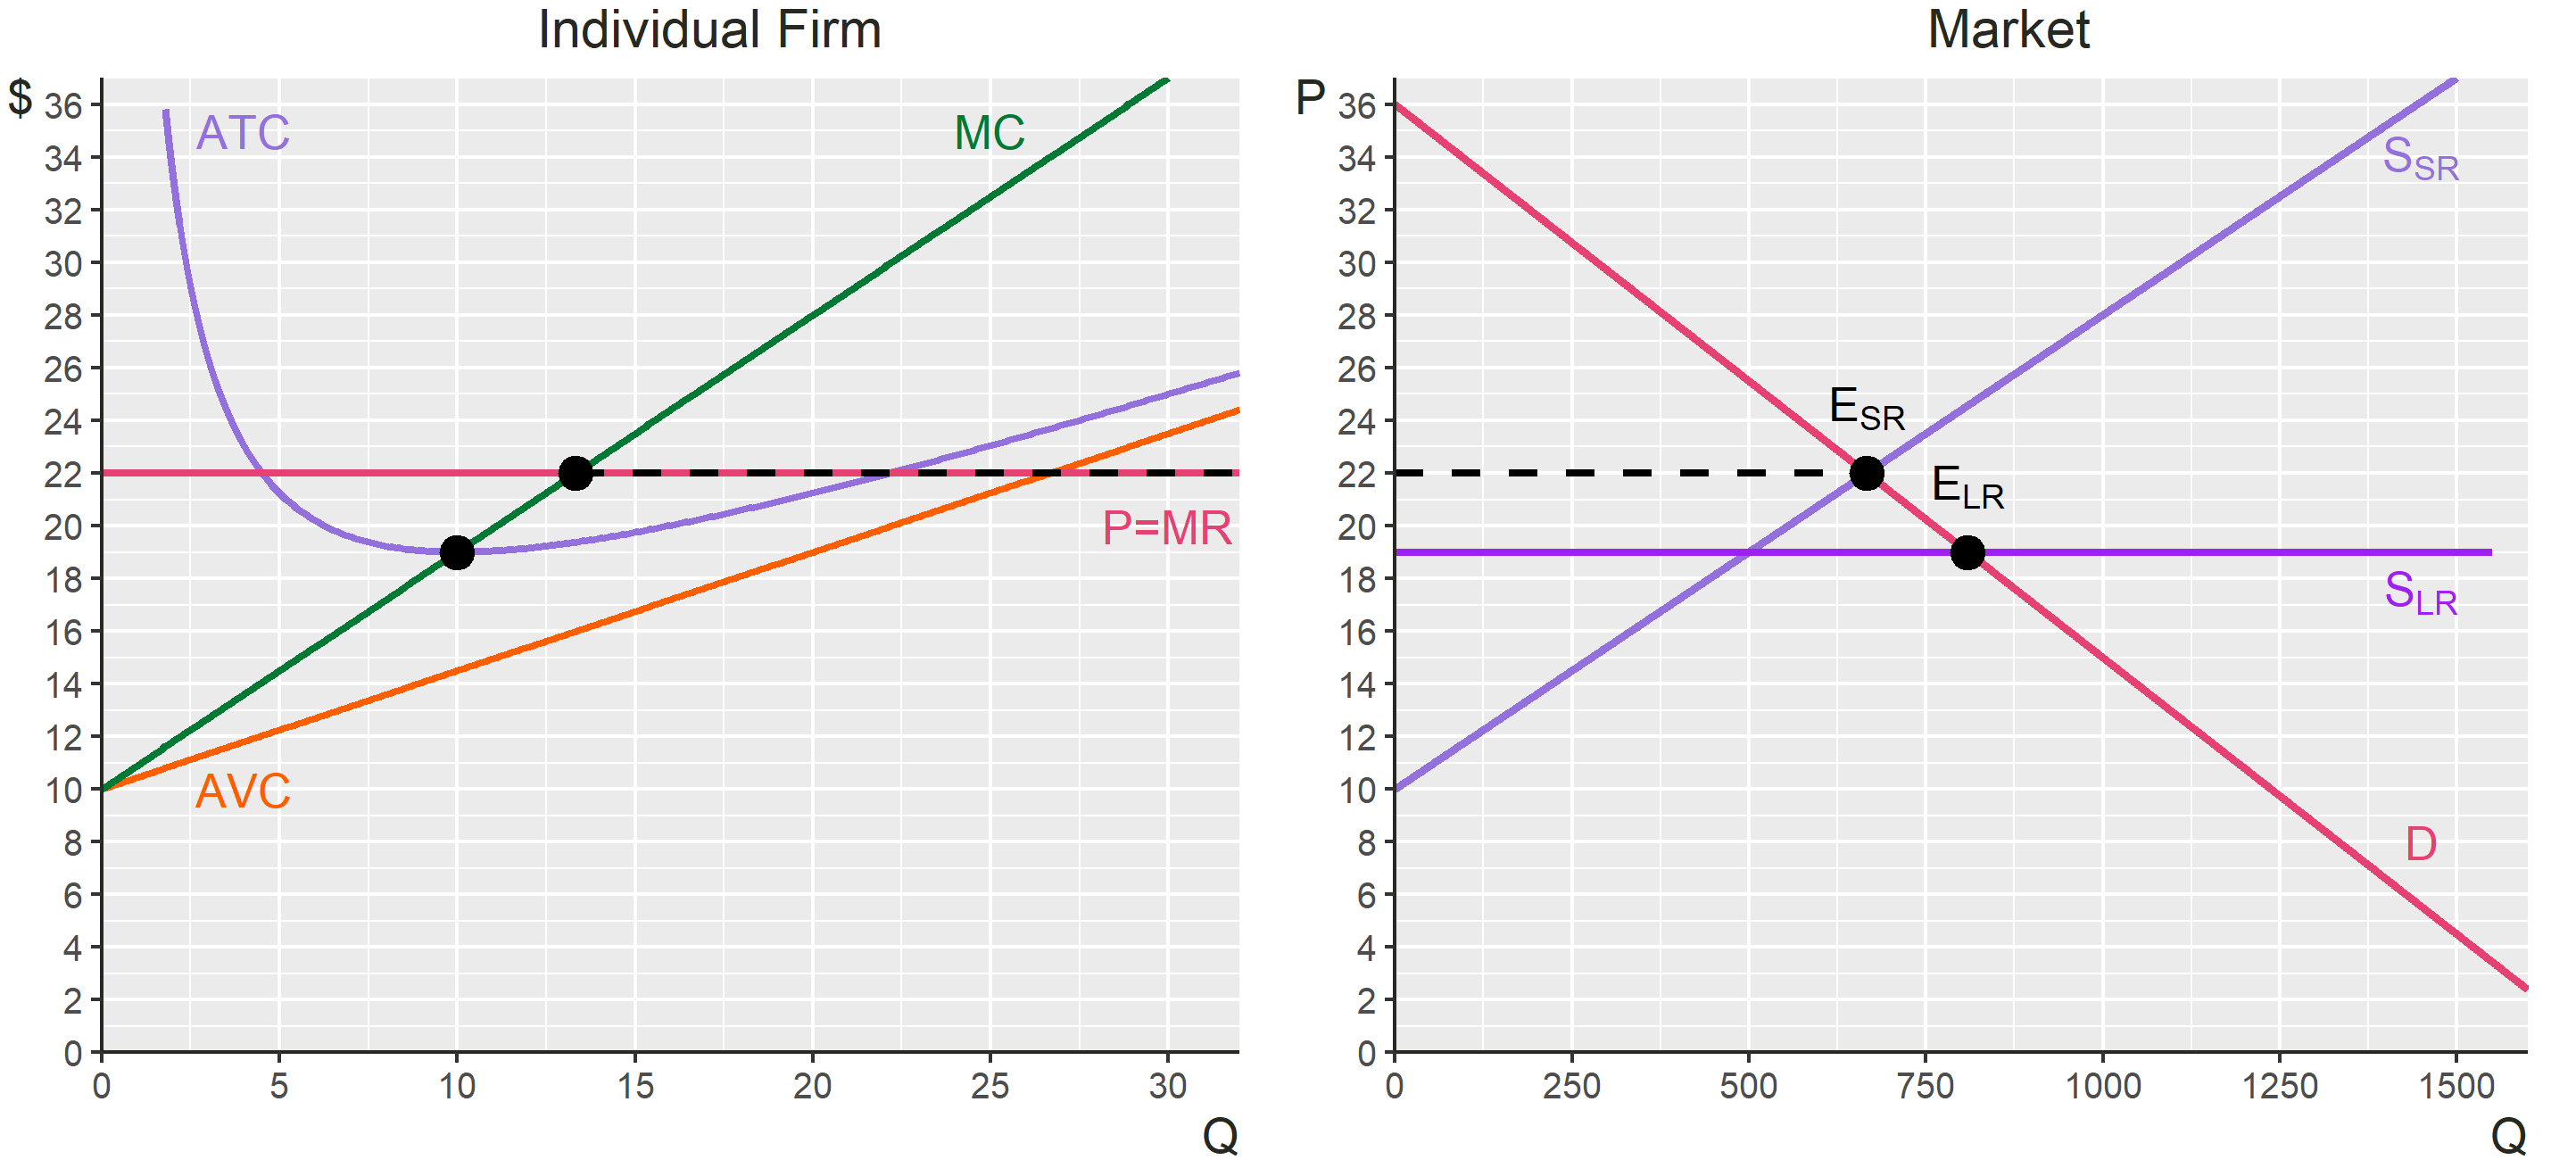
\includegraphics[width=11cm]{linex5.png}}
        \end{figure}
    \end{itemize}
\end{frame}

\begin{frame}{Equilibria}
        \begin{figure}
            \centering
            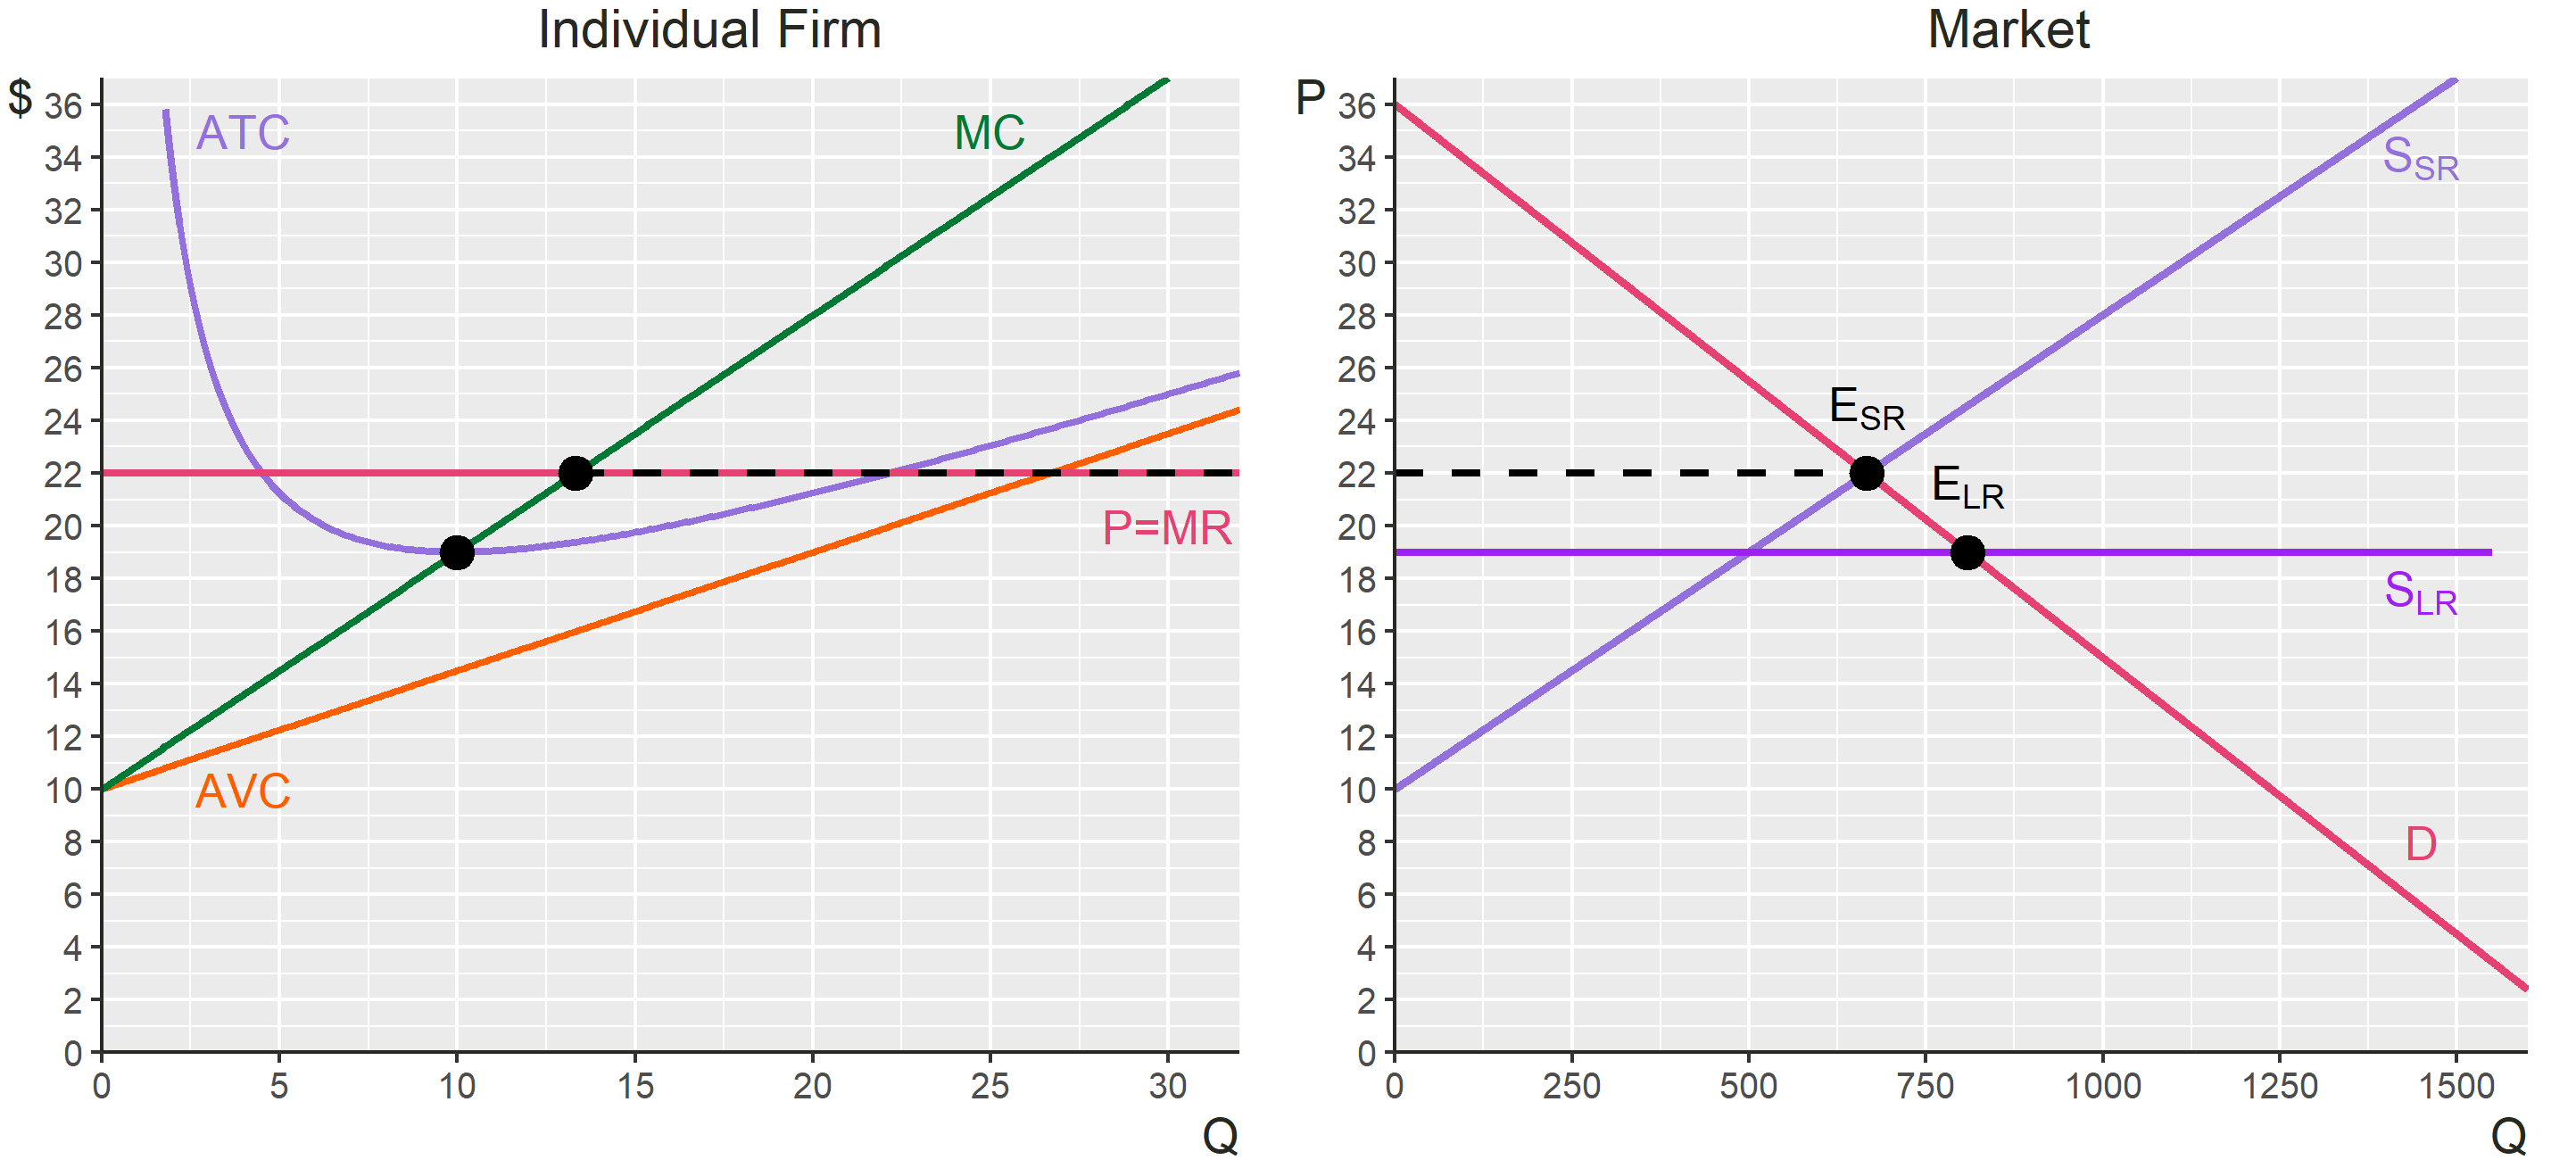
\includegraphics[width=9.5cm]{linex5.png}
        \end{figure}
    \begin{itemize}[<+->]
        \item In the short run, firms are making positive profits, so more firms enter and drive the price down
        \item In the long run, we are back to 0 profit
        \item Exactly how many firms are there in the long run?
    \end{itemize}
\end{frame}

\begin{frame}{Determining Number of Firms}
        \begin{figure}
            \centering
            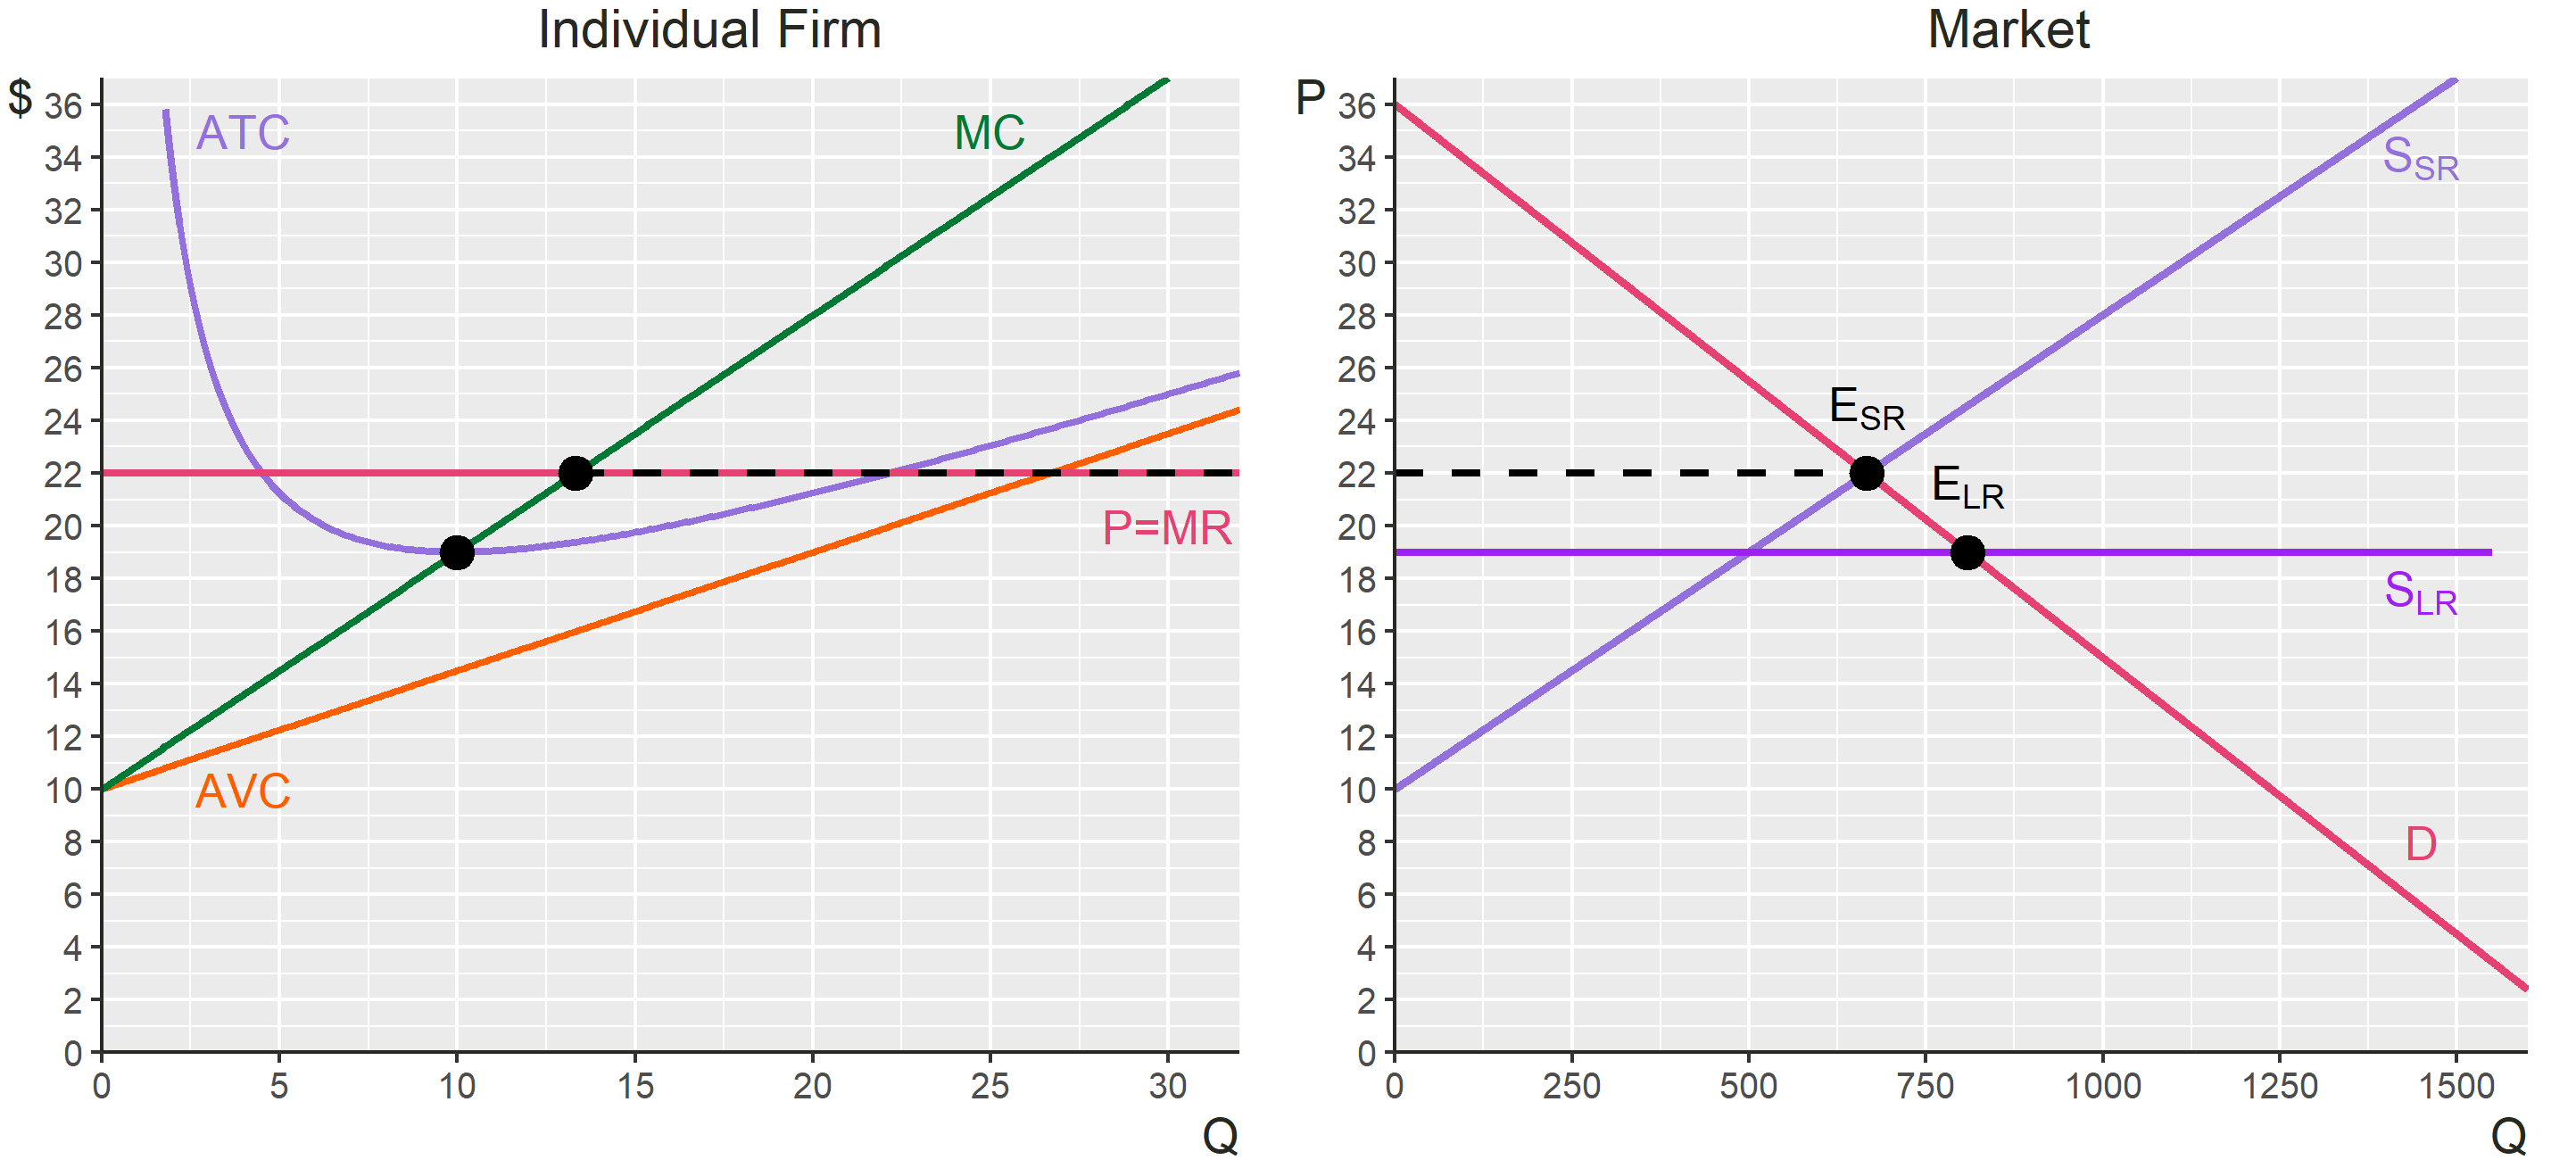
\includegraphics[width=9.5cm]{linex5.png}\vspace{-4mm}
        \end{figure}
    \begin{itemize}[<+->]
        \item Recall: to determine the number of firms, we just have to know how much each firm is producing, and the market quantity produced
        \item Example: In the above diagram, each firm is making about $13.33$ units in the short run, and the market is making about $666.66$
        \begin{itemize}
            \item As a check: $666.6\bar{6}/13.\bar{3}=50$, which is the number of firms we started with (i.e., the number of firms in the SR)
        \end{itemize}
    \end{itemize}
\end{frame}

\begin{frame}{Determining Number of Firms in the LR}
        \begin{figure}
            \centering
            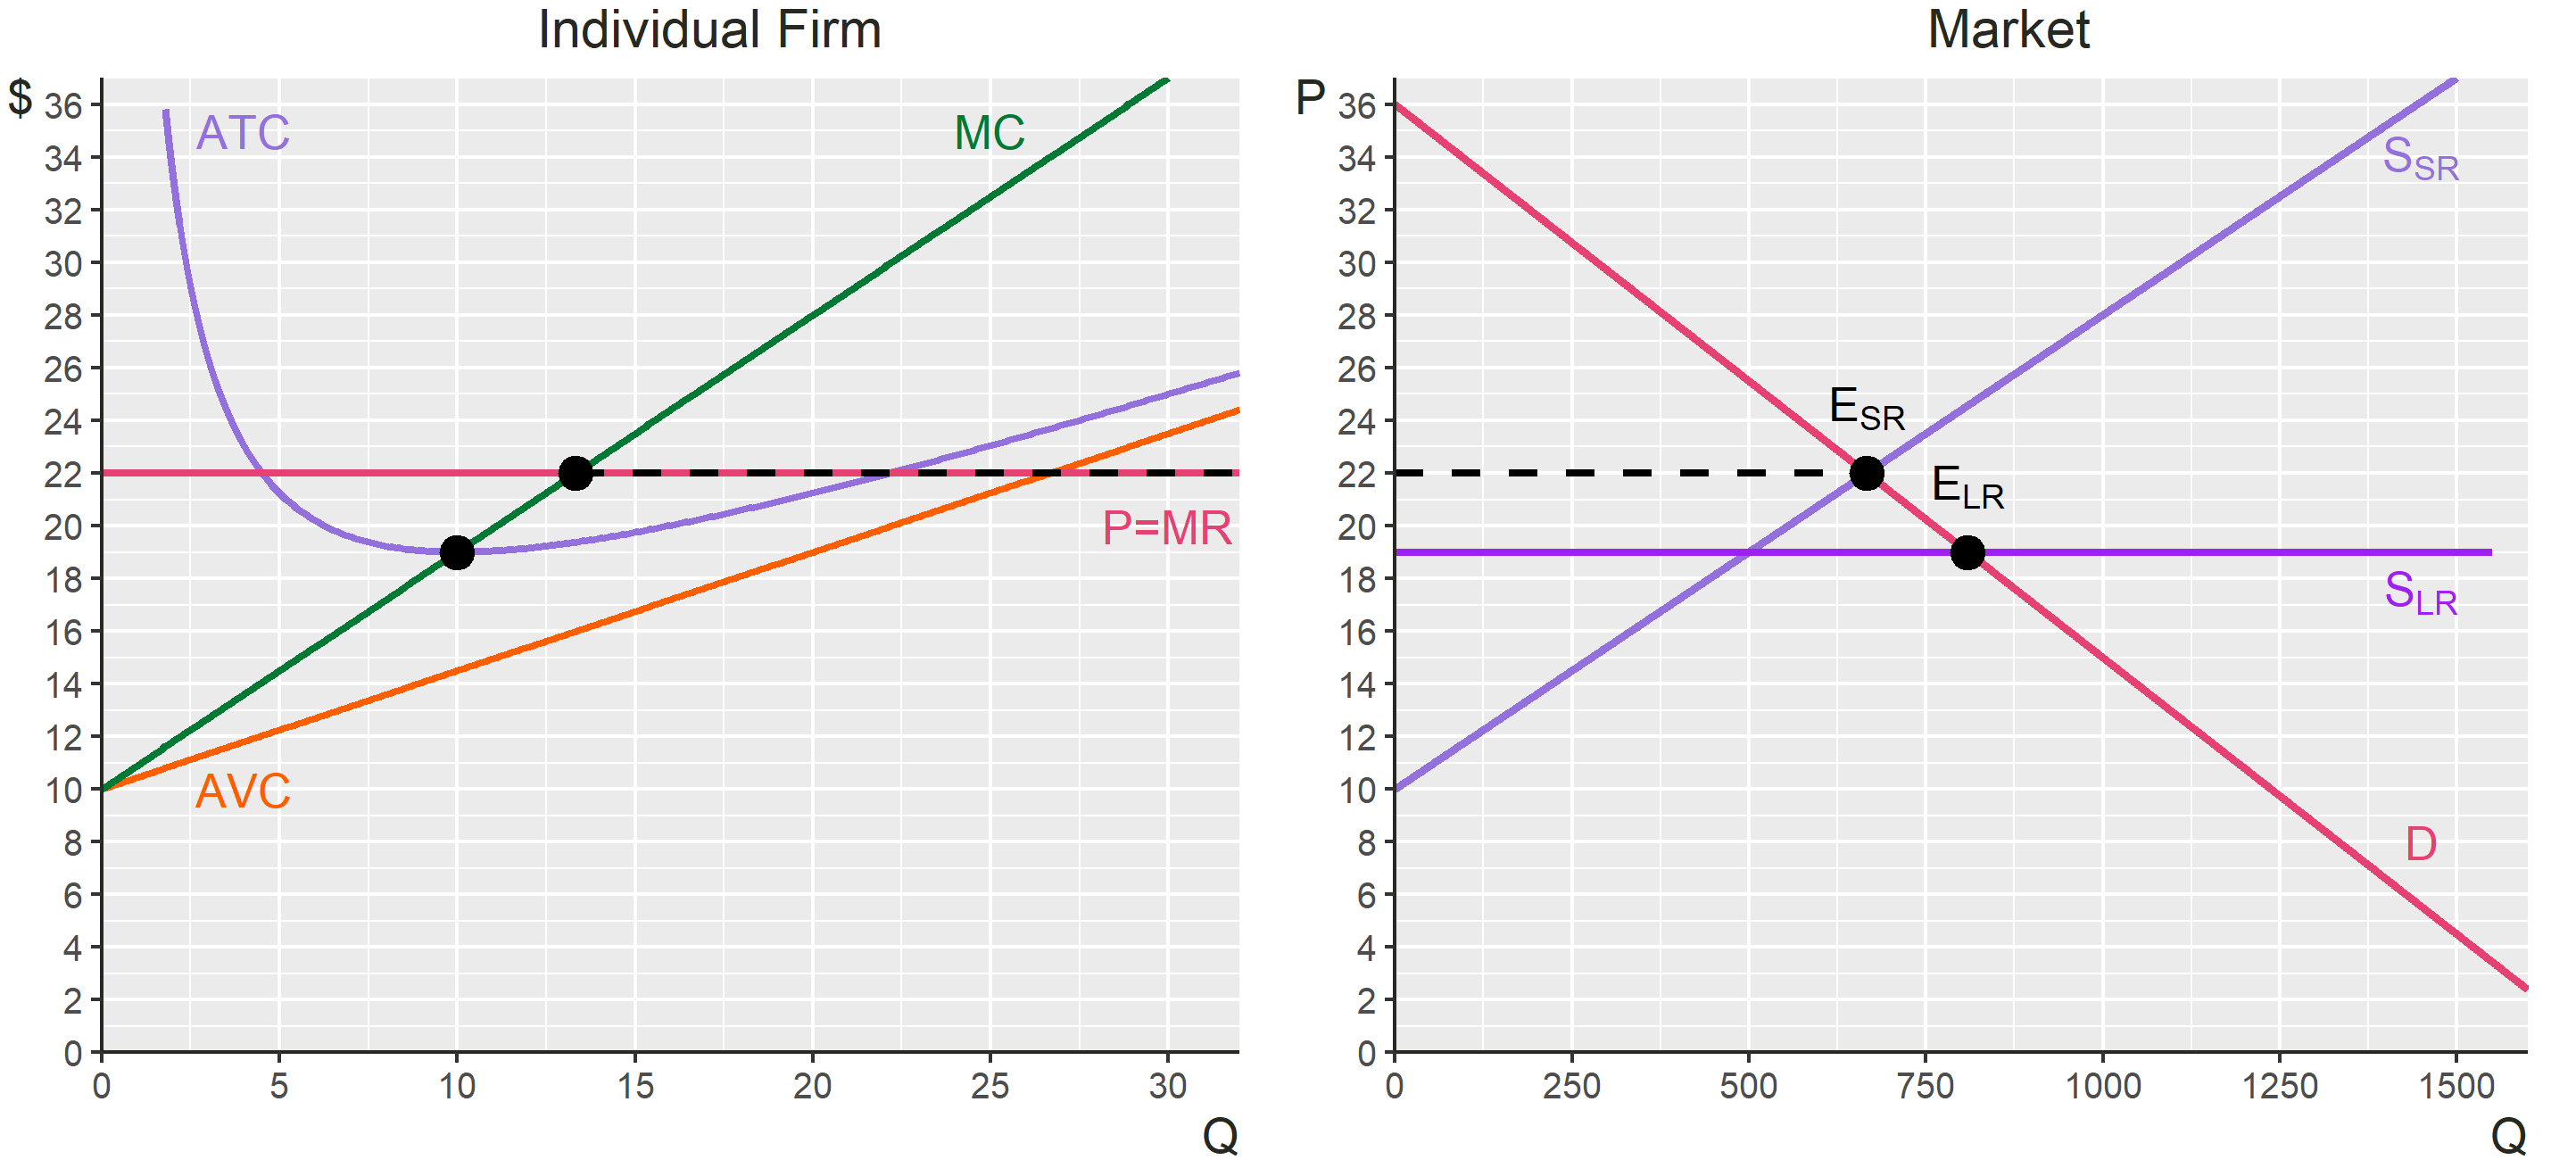
\includegraphics[width=9cm]{linex5.png}\vspace{-4mm}
        \end{figure}
    \begin{itemize}[<+->]
        \item In the previous diagram\footnote{Here, I have the numbers, so I am just giving them to you. Given an easier-to-eyeball diagram, you should be able to identify this number}, LR production in the market is about $809.524$. How much does each firm produce?
        \begin{itemize}
            \item Looking at the zero-profit point, it is 10
            \item Therefore, the number of firms in long run is 
            $$809.524/10\approx80.9\approx 81$$
        \end{itemize}
        \item So, there are 81 firms in the long run
    \end{itemize}
\end{frame}

\begin{frame}{Affects of this Demand Curve}
    \begin{itemize}[<+->]
        \item Visually, this is what happens as we transition from the short to the long run:
        \begin{figure}
            \centering
            \hbox{\hspace{0.9em}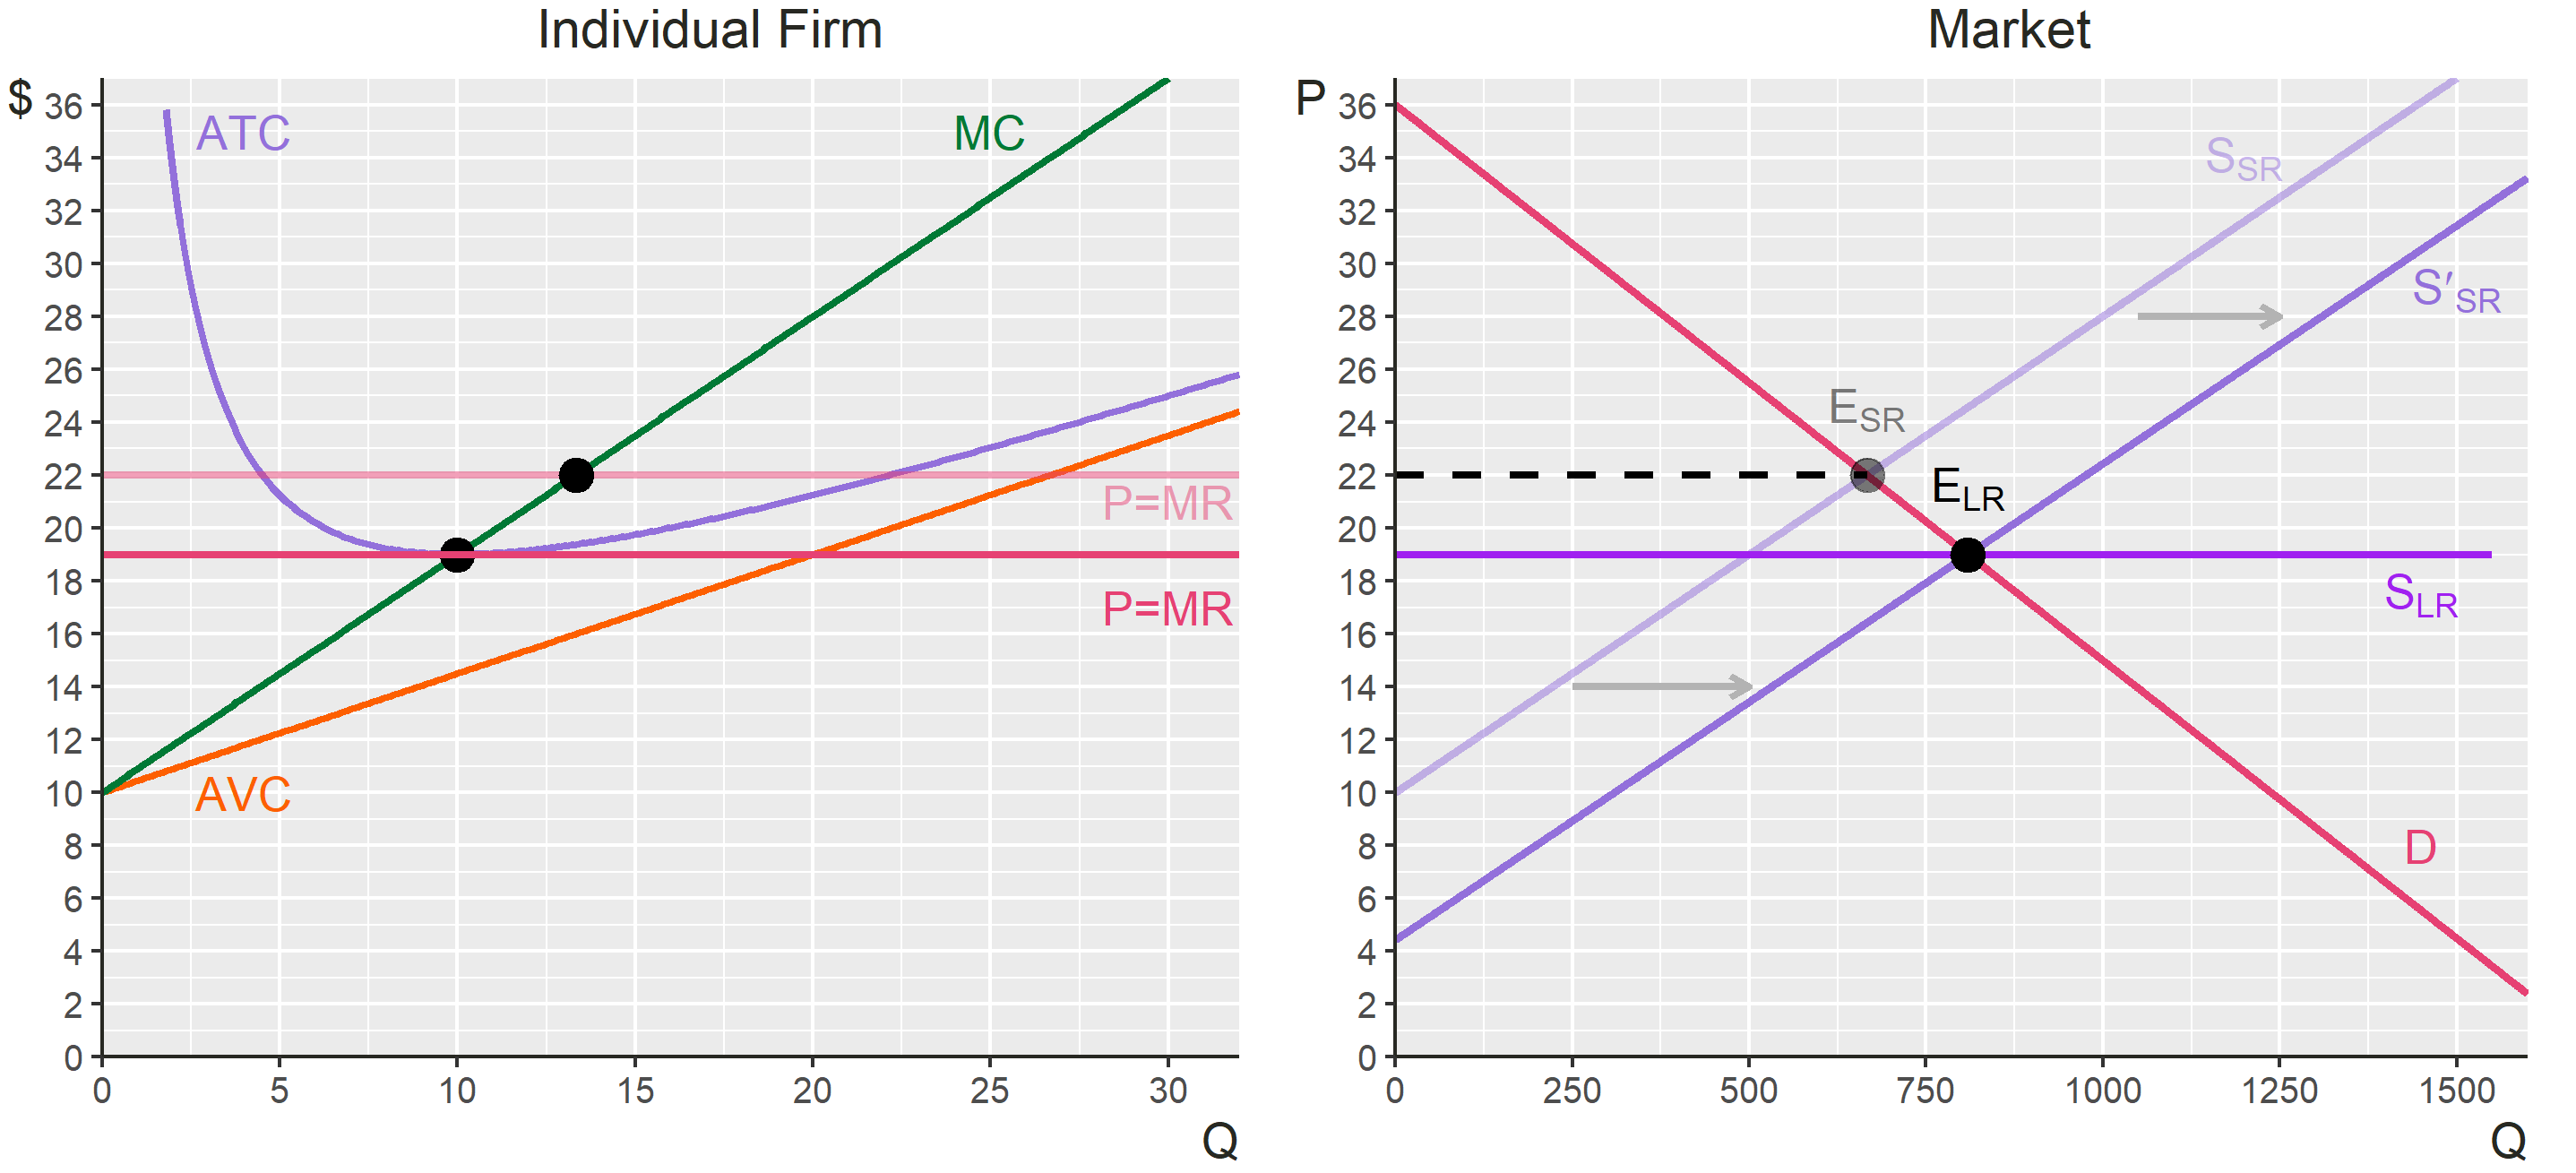
\includegraphics[width=10cm]{linex6.png}}\vspace{-4mm}
        \end{figure}
    \end{itemize}
\end{frame}

\begin{frame}{Summary}
    \begin{itemize}[<+->]
        \item There is a lot of analysis to be done here
        \item I generally won't expect you to get numbers out of this, unless I have given you nice ones
        \item My recommendation is to look at this \textbf{BEFORE YOU GO ON BREAK}, and then spend some passive time on break compartmentalizing this material, and organizing your thoughts
        \item I want you to be able to approach a problem like the one I just showed, and draw some accurate sketches with rough labels, and provide good intuition
        \begin{itemize}
            \item A great example to think about is what happens if we did this example with demand below the LR equilibrium
            \item Another good example would be shifting MC to the right, e.g. shifting supply in some way
        \end{itemize}
        \item Feel free to email me with questions next week if you are feeling hazy, or set up a meeting
    \end{itemize}
\end{frame}


\begin{frame}{How the Book Derives Optimal Profit for the Firm}
    \begin{itemize}
        \item The book carries out this discussion much differently than I have
        \item I expect you to read chapter 14 on your own, to further your understanding, and possibly gain more insights
        \item In addition to a difference in presentation style and order, I did not cover material from 14-2d or 14-3d, so read those on your own (particularly 14-3d)
        \item Also, whatever we didn't get to in class today is your responsibility to review on your own
    \end{itemize}
\end{frame}

\end{document}